\documentclass[10pt,a4paper]{article}
\usepackage[a4paper,margin=2.3cm]{geometry}
\usepackage[T1]{fontenc}
\usepackage{newpxtext,newpxmath}
\usepackage{microtype}
\usepackage{graphicx}
\usepackage{booktabs,tabularx}
\usepackage{xcolor}
\usepackage{caption,subcaption}
\usepackage{enumitem}
\usepackage{tikz}
\usetikzlibrary{arrows.meta,positioning,shapes.geometric}
\usepackage{fancyhdr}
\usepackage[section]{placeins}
\usepackage[colorlinks=true,linkcolor=blue!50!black,citecolor=blue!50!black,urlcolor=blue!50!black,
  pdftitle={What does the Super Mario 64 courtyard plaque say?},pdfauthor={mochi64},
  pdfsubject={Forward-model reconstruction of the SM64 courtyard plaque texture}]{hyperref}
\usepackage[nameinlink,capitalise]{cleveref}

\definecolor{ours}{HTML}{1B6CA8}
\captionsetup{font=small,labelfont=bf,margin=0.5em}
\setlist{nosep,leftmargin=1.4em}
\pagestyle{fancy}\fancyhf{}\renewcommand{\headrulewidth}{0.3pt}
\fancyhead[L]{\small What does the Super Mario 64 courtyard plaque say?}\fancyhead[R]{\small\thepage}

\graphicspath{{figures/}}
\newcommand{\AdobeBlur}{0.30}
\newcommand{\AdobeCanvas}{192$\times$160}
\newcommand{\AdobeDPHopeSecond}{We hope as}
\newcommand{\AdobeDPHopeSecondSse}{311.5}
\newcommand{\AdobeDPHopeTop}{We hope so}
\newcommand{\AdobeDPHopeTopSse}{311.2}
\newcommand{\AdobeDPSecond}{We hope he}
\newcommand{\AdobeDPSecondSse}{362.7}
\newcommand{\AdobeDPTop}{We hope so}
\newcommand{\AdobeDPTopSse}{362.1}
\newcommand{\AdobeEndNr}{92.7}
\newcommand{\AdobeEndOr}{117.2}
\newcommand{\AdobeEndSo}{91.4}
\newcommand{\AdobeGain}{43}
\newcommand{\AdobeGamma}{1.4}
\newcommand{\AdobeHoleE}{13.7}
\newcommand{\AdobeHoleW}{14.8}
\newcommand{\AdobeLineOne}{731.3}
\newcommand{\AdobeLineTwo}{311.2}
\newcommand{\AdobeNextTotal}{1085.1}
\newcommand{\AdobeP}{26}
\newcommand{\AdobeRatio}{4.41}
\newcommand{\AdobeTotal}{1042.5}
\newcommand{\AdobeTrack}{+2}
\newcommand{\AltABe}{459}
\newcommand{\AltABy}{420}
\newcommand{\AltAHe}{389}
\newcommand{\AltAMe}{374}
\newcommand{\AltAMy}{417}
\newcommand{\AltAWe}{355}
\newcommand{\AltBBe}{433}
\newcommand{\AltBBy}{386}
\newcommand{\AltBHe}{369}
\newcommand{\AltBMe}{359}
\newcommand{\AltBMy}{385}
\newcommand{\AltBWe}{371}
\newcommand{\AltPhABe}{Be hope us}
\newcommand{\AltPhABy}{By hope or}
\newcommand{\AltPhAHe}{He hope he}
\newcommand{\AltPhAMe}{Me hope he}
\newcommand{\AltPhAMy}{My hope he}
\newcommand{\AltPhAWe}{We hope he}
\newcommand{\AltPhBBe}{Be hope us}
\newcommand{\AltPhBBy}{By hope us}
\newcommand{\AltPhBHe}{He hope he}
\newcommand{\AltPhBMe}{Me hope he}
\newcommand{\AltPhBMy}{My hope he}
\newcommand{\AltPhBWe}{We hope he}
\newcommand{\ClaimEternalOne}{759}
\newcommand{\ClaimLieHereOne}{759}
\newcommand{\ClaimLieHereTwo}{695}
\newcommand{\ClaimLisRealAltOne}{1561}
\newcommand{\ClaimLisRealOne}{1492}
\newcommand{\ClaimLisRealStarOne}{1421}
\newcommand{\ClaimMyHopeIsLcOne}{759}
\newcommand{\ClaimMyHopeIsLcTwo}{489}
\newcommand{\ClaimMyHopeIsOne}{759}
\newcommand{\ClaimMyHopeIsTwo}{511}
\newcommand{\ClaimOursLcOne}{765}
\newcommand{\ClaimOursLcTwo}{554}
\newcommand{\ClaimOursOne}{759}
\newcommand{\ClaimOursTwo}{373}
\newcommand{\ClaimSecretStarOne}{1604}
\newcommand{\ClaimSecretStarTwo}{1126}
\newcommand{\DPBest}{343.6}
\newcommand{\DPHopeShare}{45}
\newcommand{\DescCol}{16}
\newcommand{\DescSecond}{2.0}
\newcommand{\DescVal}{5.0}
\newcommand{\EraBest}{788.7}
\newcommand{\EraN}{470}
\newcommand{\EraOther}{Schneidler Blk BT Black Italic}
\newcommand{\EraOtherSse}{926}
\newcommand{\ExBest}{734.6}
\newcommand{\ExEndN}{36,559}
\newcommand{\ExEndRank}{4}
\newcommand{\ExEndTop}{``We hope nr'' 251, ``We hope ur'' 253, ``We hope ar'' 255, ``We hope so'' 262}
\newcommand{\ExFirstN}{36,558}
\newcommand{\ExFirstRank}{8}
\newcommand{\ExFirstTop}{``Wi hope so'' 220, ``Wj hope so'' 231, ``Wf hope so'' 240, ``Wl hope so'' 243}
\newcommand{\ExMidN}{456,976}
\newcommand{\ExMidRank}{40}
\newcommand{\ExMidTop}{``We bape so'' 211, ``We bope so'' 218, ``We bupe so'' 222, ``We baps so'' 226}
\newcommand{\ExN}{949,104}
\newcommand{\ExRankStar}{14}
\newcommand{\ExStarSse}{788.7}
\newcommand{\ExTop}{Stoi 735, Stni 751, Stai 760, Slor 764, Stui 765, Stor 766}
\newcommand{\FontBest}{733.3}
\newcommand{\FontBestName}{Palatino Bold Italic (Adobe Type 1, 1990)}
\newcommand{\FontMargin}{108}
\newcommand{\FontN}{33}
\newcommand{\FontOtherBest}{841.2}
\newcommand{\FontOtherName}{N. C. Schoolbook Bold Italic (URW)}
\newcommand{\FontPalTop}{6}
\newcommand{\GameFlex}{812}
\newcommand{\GameFull}{1279}
\newcommand{\GameFullInterp}{bicubic}
\newcommand{\GameOf}{33}
\newcommand{\GameRank}{31}
\newcommand{\GameRigid}{1288}
\newcommand{\GameRigidRatio}{7.8}
\newcommand{\HSimExact}{4}
\newcommand{\HSimMaxGap}{52}
\newcommand{\HSimN}{24}
\newcommand{\HSimWordPct}{40}
\newcommand{\HopeAEAs}{111}
\newcommand{\HopeAEHe}{128}
\newcommand{\HopeAENo}{130}
\newcommand{\HopeAENr}{104}
\newcommand{\HopeAEOr}{115}
\newcommand{\HopeAESe}{99}
\newcommand{\HopeAESo}{107}
\newcommand{\HopeAEUs}{118}
\newcommand{\HopeAFBy}{244}
\newcommand{\HopeAFHe}{262}
\newcommand{\HopeAFMe}{221}
\newcommand{\HopeAFMy}{225}
\newcommand{\HopeAFWe}{198}
\newcommand{\HopeAFWi}{148}
\newcommand{\HopeAFWr}{159}
\newcommand{\HopeAFit}{45.2}
\newcommand{\HopeASize}{18}
\newcommand{\HopeATrack}{+0}
\newcommand{\HopeAVBeWithUs}{693}
\newcommand{\HopeAVByHopeSo}{443}
\newcommand{\HopeAVMyHopeIs}{473}
\newcommand{\HopeAVWeHopeHe}{361}
\newcommand{\HopeAVWeHopeNo}{343}
\newcommand{\HopeAVWeHopeOr}{359}
\newcommand{\HopeAVWeHopeSo}{366}
\newcommand{\HopeAVWeHopeUs}{351}
\newcommand{\HopeDPABest}{314.6}
\newcommand{\HopeDPABestPh}{We hops So}
\newcommand{\HopeDPARankLc}{54}
\newcommand{\HopeDPARankUc}{3}
\newcommand{\HopeDPASseLc}{350.4}
\newcommand{\HopeDPASseUc}{323.6}
\newcommand{\HopeDPUBest}{326.1}
\newcommand{\HopeDPUBestPh}{We hops So}
\newcommand{\HopeDPURankLc}{3}
\newcommand{\HopeDPURankUc}{9}
\newcommand{\HopeDPUSseLc}{328.7}
\newcommand{\HopeDPUSseUc}{338.5}
\newcommand{\HopeUEAs}{124}
\newcommand{\HopeUEHe}{124}
\newcommand{\HopeUENo}{131}
\newcommand{\HopeUENr}{91}
\newcommand{\HopeUEOr}{118}
\newcommand{\HopeUESe}{118}
\newcommand{\HopeUESo}{106}
\newcommand{\HopeUEUs}{120}
\newcommand{\HopeUFBy}{253}
\newcommand{\HopeUFHe}{230}
\newcommand{\HopeUFMe}{202}
\newcommand{\HopeUFMy}{250}
\newcommand{\HopeUFWe}{179}
\newcommand{\HopeUFWi}{181}
\newcommand{\HopeUFWr}{161}
\newcommand{\HopeUFit}{44.5}
\newcommand{\HopeUSize}{18}
\newcommand{\HopeUTrack}{+0}
\newcommand{\HopeUVBeWithUs}{680}
\newcommand{\HopeUVByHopeSo}{419}
\newcommand{\HopeUVMyHopeIs}{451}
\newcommand{\HopeUVWeHopeHe}{346}
\newcommand{\HopeUVWeHopeNo}{354}
\newcommand{\HopeUVWeHopeOr}{341}
\newcommand{\HopeUVWeHopeSo}{338}
\newcommand{\HopeUVWeHopeUs}{343}
\newcommand{\InvLisRealOne}{0.29}
\newcommand{\InvMyHopeOne}{0.74}
\newcommand{\InvMyHopeTwo}{0.68}
\newcommand{\InvOursOne}{0.74}
\newcommand{\InvOursTwo}{0.76}
\newcommand{\InvSecretOne}{0.30}
\newcommand{\InvSecretTwo}{0.44}
\newcommand{\JointADiff}{43.8}
\newcommand{\JointALo}{1176.3}
\newcommand{\JointALoLTwo}{366.0}
\newcommand{\JointAUp}{1132.5}
\newcommand{\JointAUpLTwo}{373.3}
\newcommand{\JointUDiff}{-29.7}
\newcommand{\JointULo}{1072.2}
\newcommand{\JointULoLTwo}{296.6}
\newcommand{\JointUUp}{1101.9}
\newcommand{\JointUUpLTwo}{283.0}
\newcommand{\LineTwoStone}{2172.8}
\newcommand{\LocEAFor}{158}
\newcommand{\LocEAHe}{113}
\newcommand{\LocEAIs}{140}
\newcommand{\LocEAOn}{142}
\newcommand{\LocEAOr}{118}
\newcommand{\LocEASo}{132}
\newcommand{\LocEATo}{156}
\newcommand{\LocEAUs}{127}
\newcommand{\LocEBFor}{179}
\newcommand{\LocEBHe}{114}
\newcommand{\LocEBIs}{153}
\newcommand{\LocEBOn}{154}
\newcommand{\LocEBOr}{122}
\newcommand{\LocEBSo}{134}
\newcommand{\LocEBTo}{159}
\newcommand{\LocEBUs}{123}
\newcommand{\LocEBestA}{103}
\newcommand{\LocEBestB}{96}
\newcommand{\LocFABy}{176}
\newcommand{\LocFAHe}{241}
\newcommand{\LocFAMe}{206}
\newcommand{\LocFAMy}{249}
\newcommand{\LocFANo}{275}
\newcommand{\LocFAWe}{187}
\newcommand{\LocFBBy}{194}
\newcommand{\LocFBHe}{214}
\newcommand{\LocFBMe}{190}
\newcommand{\LocFBMy}{216}
\newcommand{\LocFBNo}{271}
\newcommand{\LocFBWe}{171}
\newcommand{\LocFBestA}{171}
\newcommand{\LocFBestB}{169}
\newcommand{\SimExact}{2}
\newcommand{\SimMaxGap}{58}
\newcommand{\SimN}{24}
\newcommand{\SimTopTen}{7}
\newcommand{\SimWordPct}{47}
\newcommand{\SimWords}{32/68}
\newcommand{\StoneLegend}{2031.3}
\newcommand{\StoneLower}{881.7}
\newcommand{\StoneSD}{1.14}
\newcommand{\StoneSecret}{2087.8}
\newcommand{\StoneStar}{788.7}
\newcommand{\SwBigN}{149,699}
\newcommand{\SwBigRank}{3}
\newcommand{\SwBigTop}{Stai 760, Stor 766, Star 789, Slur 796}
\newcommand{\SwTwoN}{12,547}
\newcommand{\SwTwoRank}{1}
\newcommand{\SwTwoTop}{Star 789, Stat 895, Slot 899, Sine 922}
\newcommand{\WindowHi}{402}
\newcommand{\WindowLo}{344}

\providecommand{\FontMargin}{--}\providecommand{\FontOtherName}{--}\providecommand{\FontOtherBest}{--}\providecommand{\FontBest}{--}
\providecommand{\FontBestName}{--}\providecommand{\FontN}{--}\providecommand{\FontPalTop}{--}
\providecommand{\LocFBWe}{--}\providecommand{\LocFBestB}{--}\providecommand{\LocFABy}{--}\providecommand{\LocFAWe}{--}
\providecommand{\LocEAHe}{--}\providecommand{\LocEBHe}{--}\providecommand{\LocEASo}{--}\providecommand{\LocEBSo}{--}
\providecommand{\AltAWe}{--}\providecommand{\AltAMe}{--}\providecommand{\AltAHe}{--}\providecommand{\AltAMy}{--}\providecommand{\AltABy}{--}\providecommand{\AltABe}{--}
\providecommand{\AltPhAWe}{--}\providecommand{\AltPhAMe}{--}\providecommand{\AltPhAHe}{--}\providecommand{\AltPhAMy}{--}\providecommand{\AltPhABy}{--}\providecommand{\AltPhABe}{--}
\providecommand{\HopeUFit}{--}\providecommand{\HopeAFit}{--}\providecommand{\HopeUSize}{--}\providecommand{\HopeUTrack}{--}
\providecommand{\HopeUFWe}{--}\providecommand{\HopeUFMe}{--}\providecommand{\HopeUFWr}{--}\providecommand{\HopeUESo}{--}\providecommand{\HopeUEOr}{--}
\providecommand{\HopeUEUs}{--}\providecommand{\HopeUEHe}{--}\providecommand{\HopeAESo}{--}\providecommand{\HopeAEOr}{--}\providecommand{\HopeAEUs}{--}
\providecommand{\HopeUVWeHopeSo}{--}\providecommand{\HopeUVWeHopeOr}{--}\providecommand{\HopeUVWeHopeUs}{--}\providecommand{\HopeUVWeHopeHe}{--}
\providecommand{\HopeDPURankLc}{--}\providecommand{\HopeDPUSseLc}{--}\providecommand{\HopeDPARankUc}{--}
\providecommand{\HSimN}{--}\providecommand{\HSimExact}{--}\providecommand{\HSimMaxGap}{--}\providecommand{\HSimWordPct}{--}
\providecommand{\JointAUp}{--}\providecommand{\JointALo}{--}\providecommand{\JointUUp}{--}\providecommand{\JointULo}{--}
\providecommand{\WindowLo}{--}\providecommand{\WindowHi}{--}
\providecommand{\ClaimLisRealOne}{--}\providecommand{\ClaimLisRealAltOne}{--}
\providecommand{\GameRigid}{--}\providecommand{\GameFull}{--}\providecommand{\GameRigidRatio}{--}\providecommand{\GameRank}{--}\providecommand{\GameOf}{--}\providecommand{\GameFlex}{812}
\providecommand{\InvOursOne}{--}\providecommand{\InvOursTwo}{--}\providecommand{\InvLisRealOne}{--}\providecommand{\InvSecretOne}{--}\providecommand{\InvSecretTwo}{--}\providecommand{\InvMyHopeTwo}{--}\providecommand{\InvMyHopeOne}{--}
\providecommand{\StoneStar}{--}\providecommand{\StoneLower}{--}\providecommand{\StoneLegend}{--}\providecommand{\StoneSecret}{--}\providecommand{\SwTwoN}{--}\providecommand{\SwTwoRank}{--}\providecommand{\SwTwoTop}{--}\providecommand{\SwBigN}{--}\providecommand{\SwBigRank}{--}\providecommand{\SwBigTop}{--}\providecommand{\ExN}{--}\providecommand{\ExRankStar}{--}\providecommand{\ExStarSse}{--}\providecommand{\ExBest}{--}\providecommand{\ExTop}{--}\providecommand{\ExFirstN}{--}\providecommand{\ExFirstRank}{--}\providecommand{\ExFirstTop}{--}\providecommand{\ExEndN}{--}\providecommand{\ExEndRank}{--}\providecommand{\ExEndTop}{--}\providecommand{\ExMidN}{--}\providecommand{\ExMidRank}{--}\providecommand{\ExMidTop}{--}\providecommand{\EraN}{--}\providecommand{\EraBest}{--}\providecommand{\EraOther}{--}\providecommand{\EraOtherSse}{--}
\providecommand{\NgOneRigid}{--}\providecommand{\NgOneKern}{--}\providecommand{\NgOneGain}{--}\providecommand{\NgOneNoise}{--}\providecommand{\NgTwoRigid}{--}\providecommand{\NgTwoKern}{--}\providecommand{\NgTwoGain}{--}\providecommand{\NgTwoNoise}{--}\providecommand{\DzPlain}{--}\providecommand{\DzKern}{--}\providecommand{\DzNormal}{--}\providecommand{\DzScreen}{--}\providecommand{\DzLighten}{--}\providecommand{\DzBlendGain}{--}\providecommand{\DzBlendNoise}{--}\providecommand{\DzShadowGain}{--}\providecommand{\DzShadowNoise}{--}\providecommand{\DzEmbossGain}{--}\providecommand{\DzEmbossNoise}{--}\providecommand{\DzOutlineGain}{--}\providecommand{\DzOutlineNoise}{--}\providecommand{\DzSharpenGain}{--}\providecommand{\DzSharpenNoise}{--}\providecommand{\DzLineGain}{--}\providecommand{\DzLineNoise}{--}\providecommand{\DzScaleInt}{--}\providecommand{\DzScaleBest}{--}\providecommand{\DzScaleW}{--}\providecommand{\DzScaleH}{--}\providecommand{\DzScaleGain}{--}\providecommand{\DzScaleNoise}{--}
\providecommand{\AdobeLineOne}{--}\providecommand{\AdobeLineTwo}{--}\providecommand{\AdobeTotal}{--}\providecommand{\AdobeNextTotal}{--}\providecommand{\AdobeGain}{--}
\providecommand{\AdobeHoleW}{--}\providecommand{\AdobeHoleE}{--}\providecommand{\AdobeDPTop}{--}\providecommand{\AdobeDPTopSse}{--}\providecommand{\AdobeDPSecond}{--}
\providecommand{\AdobeDPHopeTop}{--}\providecommand{\AdobeDPHopeTopSse}{--}\providecommand{\AdobeDPHopeSecond}{--}\providecommand{\AdobeEndSo}{--}\providecommand{\AdobeEndNr}{--}
\providecommand{\AdobeCanvas}{--}\providecommand{\AdobeP}{--}\providecommand{\AdobeTrack}{--}\providecommand{\AdobeGamma}{--}\providecommand{\AdobeBlur}{--}\providecommand{\AdobeRatio}{--}
\providecommand{\DescCol}{16}\providecommand{\DescVal}{--}\providecommand{\StoneSD}{--}\providecommand{\DescSecond}{--}

\newcommand{\q}[1]{``#1''}
\newcommand{\SSE}{\textsc{sse}}

\title{\vspace{-1.2cm}\textbf{What does the Super Mario 64 courtyard plaque say?}\\[0.3em]
\large A forward-model reconstruction of the \q{L is real 2401} texture: font, process and text}
\author{mochi64}
\date{14 October 2026}

\begin{document}
\maketitle
\thispagestyle{empty}

\begin{abstract}
\noindent The stone plaque on the star statue in the castle courtyard of \emph{Super Mario 64} (1996) has fuelled one of the longest-running
legends in gaming: that it reads \q{L is real 2401}. The plaque is a single $32{\times}32$ grey texture with two lines of
text about three to five pixels tall, which is far below the resolution needed to read letters by eye. Instead of
enhancing or interpreting the image, we \emph{simulate} how a 1996 artist would have produced it. We type a candidate
text in a real period font, resize it into the texture with a standard filter, and measure how well the result matches
the stored pixels after removing the stone background. We do this for millions of candidate texts, fonts and process
settings on a GPU, and calibrate the method on synthetic plaques with known text.
We find that
(i)~the text is set in \textbf{Palatino Bold Italic}, most likely Adobe's own 1990 PostScript Type~1 version as used
with Adobe Type Manager; it beats every
other era font family under an identical, exhaustive process search, including the game's own dialog font, which is
clearly ruled out;
(ii)~a \emph{single rigid designer pipeline} reproduces the texture: with Adobe's file 192$\times$160 artwork,
26\,px type, bilinear resize, light blur and gamma~1.4; the Apple and URW Palatinos independently converge on
160$\times$128, 23\,px and gamma~1.8. A second pass against the extracted plain stone, an exhaustive test of every
3--4-letter string and \EraN{} era fonts (including everything an SGI workstation could install) changes nothing;
working like the designer (hand kerning, a 1\,\% narrower 190$\times$160 artwork) brings the model to within about one
grey level of the plaque, and the few pixels left look hand-retouched;
(iii)~line~1 reads \textbf{\q{Eternal Star}}: \q{Star} is the best of 27{,}122 words as the second word (whether
the s is upper or lower case cannot be decided);
(iv)~line~2 is set in the same process at 17--18\,px, centred under line~1, and \q{hope} is the best of 12{,}556
middle words. We then fitted line~2's own typesetting on the four letters of \q{hope} alone. On their own, held-out
pixels, \q{We} becomes the best first word and \q{so} the best real ending, and the unconstrained dictionary search
returns \q{We hope so} among its top three strings.
With Adobe's original Palatino, a blind search over 17.7k words returns exactly \q{We hope so} as its best string.
Our most likely reading is therefore
\begin{center}\Large\textit{Eternal Star}\\\textit{We hope so}\end{center}
\q{L is real 2401}, \q{A Secret star / lie here\,\textasciitilde}, \q{My hope is} and other published readings fit
the pixels substantially worse under the same model. All code, results and figures are released for independent
verification; no Nintendo data is redistributed.
\end{abstract}

\tableofcontents
\clearpage

%======================================================================================================
\section{Introduction}
In the courtyard behind Princess Peach's castle stands a statue topped by a star, with a small engraved plaque at its base
(\cref{fig:texture}). The plaque is blurry, and for almost three decades players have argued about what it says.
\begin{itemize}
\item \textbf{\q{L is real 2401}.} This is the classic reading from the late 1990s, taken as a hint that Luigi was
hidden in the game~\cite{smwcourtyard,mysteries}. A variant spells the number as \q{2041}~\cite{moby}.
\item \textbf{The 1998 Nintendo letter.} A Nintendo of America game-play counsellor's letter from 1998, which surfaced
in 2016, called the plaque a developers' joke without saying what it reads~\cite{mnn,sora}.
\item \textbf{\q{Eternal Star}.} This is the reading the Super Mario Wiki considers \q{more likely}, set \q{in a heavily
serifed font}~\cite{smwcourtyard}.
\item \textbf{\q{A Secret star / lie here\,\textasciitilde}.} Daniel Nodd (No64DD) proposed this in 2015 from
photographs of CRT screens, and Nintendo Life covered it in 2019~\cite{nlife}.
\item \textbf{\q{My hope is}.} A further suggestion for line~2, based on two descenders and an ascender.
\end{itemize}

All previous attempts share one weakness. They \emph{read} a 32$\times$32 image, whether by eye, by upscaling or by
photographing a CRT, and people then disagree about which shapes they see. At this resolution a human (or an
upscaler) will find whatever text they are primed to find. This report takes the opposite approach.
\begin{enumerate}
\item \textbf{Model, don't read.} We write down how such a texture is made: type, resize, blur, gamma, on top of a stone
background.
\item \textbf{Score hypotheses.} Every candidate (font, process, text) is rendered through that model and compared with
the stored pixels.
\item \textbf{Calibrate.} Synthetic plaques with known text show what the method can and cannot recover.
\end{enumerate}
We only use the texture as it ships in the game. Leaked source material is not used.

%======================================================================================================
\section{The data}
\label{sec:data}
The plaque is the texture \texttt{castle\_grounds\_textures.08800}. It is a $32{\times}32$ RGBA16 texture inside the
MIO0-compressed \texttt{outside} texture segment, mapped onto a quad of about $142{\times}105$ world units in the
courtyard model.
\begin{itemize}
\item We extracted it from the US, Japanese, European and Shindou ROMs, using segment offsets from the public
decompilation~\cite{decomp}.
\item It is \textbf{byte-identical in all versions} (SHA-1 \texttt{88ef618a\ldots}), so the text was never localised
or revised.
\item The texture is pure grey and uses only 23 distinct 5-bit levels.
\end{itemize}

There are two lines of text:
\begin{itemize}
\item \textbf{line 1:} rows 8--12, columns 2--29;
\item \textbf{line 2:} mainly rows 17--19, columns 7--23;
\item the lower rows are clean stone.
\end{itemize}

\begin{figure}[t]\centering
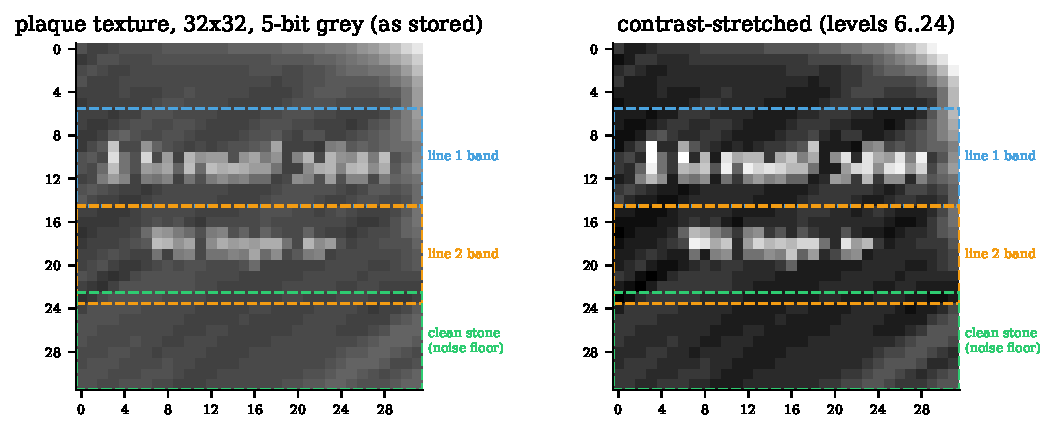
\includegraphics[width=\linewidth]{texture.pdf}
\caption{The plaque texture as stored in the ROM (left) and contrast-stretched (right). Dashed boxes mark the two text
bands we model and the clean stone rows that define the noise floor.}
\label{fig:texture}
\end{figure}

%======================================================================================================
\section{Method: a forward model of the designer's process}
\label{sec:model}

\paragraph{Why direct reading fails.}
At 1.5--2 texture pixels per character, many different strings produce almost the same blur. In early experiments we
let every letter move and change freely. Meaningless strings then fitted \emph{as well as or better than} any real
sentence, which shows that pixel evidence alone cannot identify the text. Identification only becomes possible once the
\emph{process} is constrained by the way the texture was actually made.

\paragraph{Generative model.}
We model the stored texture $t$ as
\[ t \;=\; \text{stone} \;+\; L\cdot\big(\,\mathcal{R}(\text{text})\,\big)^{\gamma} \;+\; \text{noise}, \]
where $\mathcal{R}$ is the designer's rendering process (\cref{fig:pipeline}):
\begin{enumerate}
\item The text is typed \emph{once}, anti-aliased, with font $F$ at an integer pixel size $P$, with tracking, optional
pair kerning, and fractional or whole-pixel advances.
\item It is typed on an artwork canvas of $32k_x\times32k_y$ pixels.
\item The canvas is resized to $32\times32$ with a standard filter (nearest, box, bilinear, bicubic, Lanczos), whose
support is scaled with the downsampling factor as in Photoshop and PIL.
\item An optional Gaussian blur is applied, then a gamma $\gamma$.
\end{enumerate}
The engraving brightness $L$ is solved in closed form.

The stone is a nuisance. Inside each $4$-column block of a text band it is modelled as a plane ($a+bx+cy$) and projected
out exactly, so the score is the residual sum of squares (\SSE) after the best plane and the best ink level.

\paragraph{Honest noise floor.}
Applying the identical operator to the nine clean stone rows 23--31 gives \SSE{}~$=165.7$. This is what pure stone
texture with no text costs. No model can be expected to go far below a few times this value, because the stone under
the letters is unknown.

\paragraph{Search.}
All renderings are expressed as matrix products: canvas$\to$texture weight matrices, with every integer position as a
slice. This makes exhaustive searches feasible on one consumer GPU (RTX~2060\,S): millions of configurations per second
for line~1, and a K-best dynamic programme over word sequences for line~2 (\cref{sec:line2}).

\begin{figure}[t]\centering
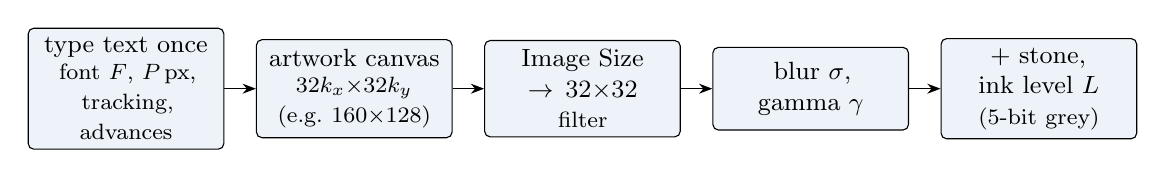
\begin{tikzpicture}[node distance=4mm, box/.style={draw,rounded corners=2pt,fill=ours!8,align=center,font=\small,minimum height=1.05cm,text width=2.25cm}, >=Stealth]
\node[box] (a) {type text once\\ \footnotesize font $F$, $P$\,px,\\ tracking, advances};
\node[box,right=of a] (b) {artwork canvas\\ \footnotesize $32k_x{\times}32k_y$\\ (e.g.\ 160$\times$128)};
\node[box,right=of b] (c) {Image Size\\ $\to 32{\times}32$\\ \footnotesize filter};
\node[box,right=of c] (d) {blur $\sigma$,\\ gamma $\gamma$};
\node[box,right=of d] (e) {$+$ stone,\\ ink level $L$\\ \footnotesize (5-bit grey)};
\draw[->] (a)--(b); \draw[->] (b)--(c); \draw[->] (c)--(d); \draw[->] (d)--(e);
\end{tikzpicture}
\caption{The designer pipeline we simulate. Every step is a single global setting. There are no per-letter adjustments.}
\label{fig:pipeline}
\end{figure}

%======================================================================================================
\section{Identifying the font}
\label{sec:font}
The first question is which typeface the artist used. We restricted ourselves to fonts that existed in 1995--96 and that
a Nintendo artist could plausibly have had:
\begin{itemize}
\item Macintosh system and LaserWriter fonts: Apple System~7.5.3 Palatino and Times, New~York;
\item Adobe PostScript fonts: IRIX~5.3 Type~1, plus X11 Adobe bitmap fonts;
\item Microsoft's 1996 core fonts;
\item classic Mac bitmap fonts with QuickDraw styles;
\item the game's own dialog font, extracted from the ROM;
\item free metric-compatible clones of the 35 PostScript fonts (URW base35).
\end{itemize}
Modern fonts were excluded.

\paragraph{Tournament ($\approx$\,530 fonts and variants).}
A flexible model first screened 393 font files, then refined the best 157. It was flexible in that it allowed scale,
aspect, blur, gamma and small per-letter shifts. The best member of each family is shown in \cref{fig:fontsflex}.
\begin{itemize}
\item \textbf{Palatino wins clearly} (554), ahead of Times (638), New Century Schoolbook (694) and Georgia (745).
\item The SM64 dialog font (812), Helvetica/Arial (890) and all others are far behind.
\item Within Palatino, the 1980s/1990s design (URW P052, Apple 1996, Adobe 1990) fits better than the revised Palatino
Linotype of 1998/99, which scores 633.
\end{itemize}

\begin{figure}[t]\centering
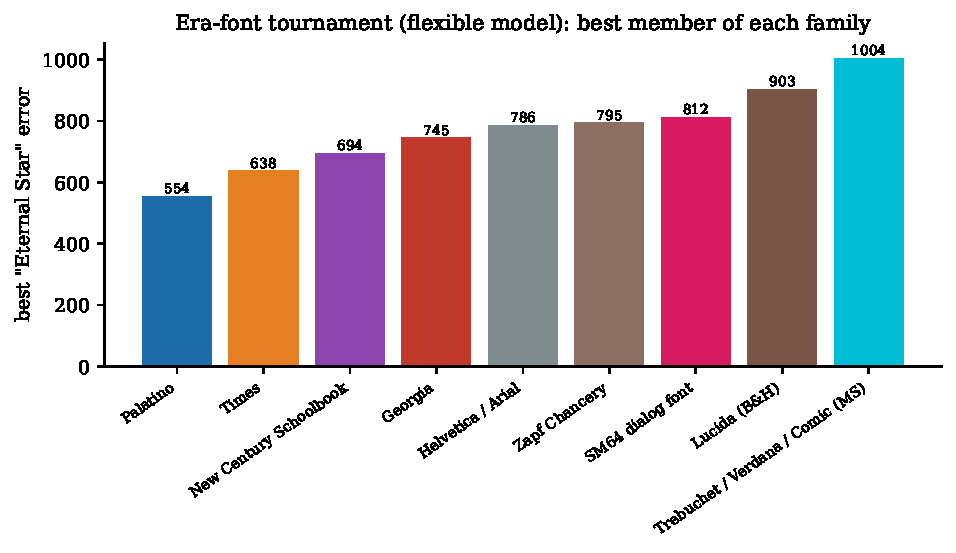
\includegraphics[width=0.92\linewidth]{fonts_flexible.pdf}
\caption{Era-font tournament, flexible model: the best \q{Eternal Star} error of each font family.}
\label{fig:fontsflex}
\end{figure}

\paragraph{Identical rigid process search for every family.}
The flexible model could favour fonts with odd spacing, so we repeated the comparison with the \emph{rigid} designer
model. Every font received exactly the same exhaustive search over the following settings:
\begin{itemize}
\item 4 canvas shapes and 10 sizes;
\item tracking, kerning and two advance modes;
\item 4 word spaces, 2 filters, 2 blurs and 4 gammas;
\item all positions.
\end{itemize}
\Cref{fig:fontsrigid} and \cref{tab:fontsrigid} show the result. The best font is \FontBestName{} (\SSE~\FontBest), and
the best non-Palatino font, \FontOtherName{}, is \FontMargin{} worse. \Cref{fig:fontpanels} shows what each family's best
recipe actually prints: only the Palatino italics reproduce the narrow, slanted, high-contrast letters of the real
plaque.

\begin{figure}[p]\centering
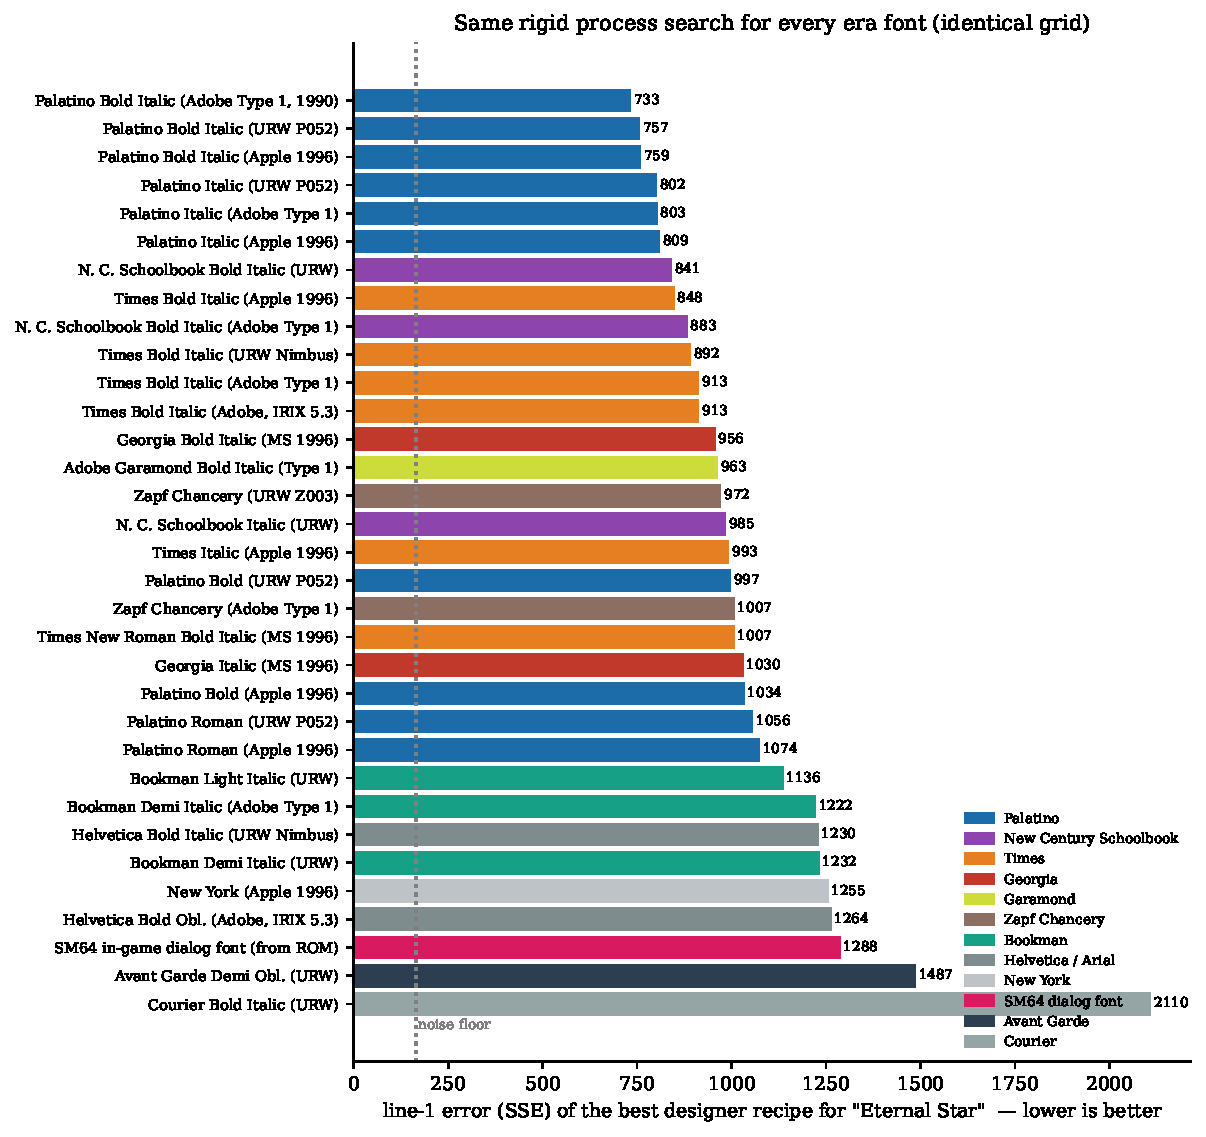
\includegraphics[width=\linewidth]{fonts_rigid.pdf}
\caption{Same rigid process search for \FontN{} era fonts: the best \q{Eternal Star} error per font, coloured by family.}
\label{fig:fontsrigid}
\end{figure}
\begin{table}[p]\centering\small
\IfFileExists{tables/fonts_rigid.tex}{\begin{tabular}{rllrr}\toprule
\# & font & family & SSE & $\Delta$ to best \\ \midrule
1 & Palatino Bold Italic (Adobe Type 1, 1990) & Palatino & 733.3 & +0.0 \\
2 & Palatino Bold Italic (URW P052) & Palatino & 756.9 & +23.6 \\
3 & Palatino Bold Italic (Apple 1996) & Palatino & 759.2 & +25.9 \\
4 & Palatino Italic (URW P052) & Palatino & 801.6 & +68.3 \\
5 & Palatino Italic (Adobe Type 1) & Palatino & 802.9 & +69.6 \\
6 & Palatino Italic (Apple 1996) & Palatino & 809.1 & +75.9 \\
7 & N. C. Schoolbook Bold Italic (URW) & New Century Schoolbook & 841.2 & +108.0 \\
8 & Times Bold Italic (Apple 1996) & Times & 847.9 & +114.6 \\
9 & N. C. Schoolbook Bold Italic (Adobe Type 1) & New Century Schoolbook & 882.6 & +149.3 \\
10 & Times Bold Italic (URW Nimbus) & Times & 891.8 & +158.5 \\
11 & Times Bold Italic (Adobe Type 1) & Times & 913.4 & +180.1 \\
12 & Times Bold Italic (Adobe, IRIX 5.3) & Times & 913.4 & +180.1 \\
13 & Georgia Bold Italic (MS 1996) & Georgia & 956.1 & +222.8 \\
14 & Adobe Garamond Bold Italic (Type 1) & Garamond & 963.2 & +230.0 \\
15 & Zapf Chancery (URW Z003) & Zapf Chancery & 971.6 & +238.4 \\
16 & N. C. Schoolbook Italic (URW) & New Century Schoolbook & 984.5 & +251.3 \\
17 & Times Italic (Apple 1996) & Times & 992.8 & +259.5 \\
18 & Palatino Bold (URW P052) & Palatino & 997.0 & +263.7 \\
19 & Zapf Chancery (Adobe Type 1) & Zapf Chancery & 1007.4 & +274.1 \\
20 & Times New Roman Bold Italic (MS 1996) & Times & 1007.5 & +274.2 \\
21 & Georgia Italic (MS 1996) & Georgia & 1030.4 & +297.1 \\
22 & Palatino Bold (Apple 1996) & Palatino & 1033.8 & +300.6 \\
23 & Palatino Roman (URW P052) & Palatino & 1056.3 & +323.1 \\
24 & Palatino Roman (Apple 1996) & Palatino & 1074.3 & +341.1 \\
25 & Bookman Light Italic (URW) & Bookman & 1136.5 & +403.2 \\
26 & Bookman Demi Italic (Adobe Type 1) & Bookman & 1222.0 & +488.8 \\
27 & Helvetica Bold Italic (URW Nimbus) & Helvetica / Arial & 1229.8 & +496.5 \\
28 & Bookman Demi Italic (URW) & Bookman & 1232.4 & +499.1 \\
29 & New York (Apple 1996) & New York & 1255.2 & +521.9 \\
30 & Helvetica Bold Obl. (Adobe, IRIX 5.3) & Helvetica / Arial & 1263.6 & +530.3 \\
31 & SM64 in-game dialog font (from ROM) & SM64 dialog font & 1288.0 & +554.7 \\
32 & Avant Garde Demi Obl. (URW) & Avant Garde & 1486.7 & +753.4 \\
33 & Courier Bold Italic (URW) & Courier & 2109.6 & +1376.3 \\
\bottomrule\end{tabular}
}{(table generated by \texttt{plaquedecode figures})}
\caption{Font ranking under the identical rigid process search (\SSE{} of the best recipe for \q{Eternal Star}).}
\label{tab:fontsrigid}
\end{table}
\begin{figure}[p]\centering
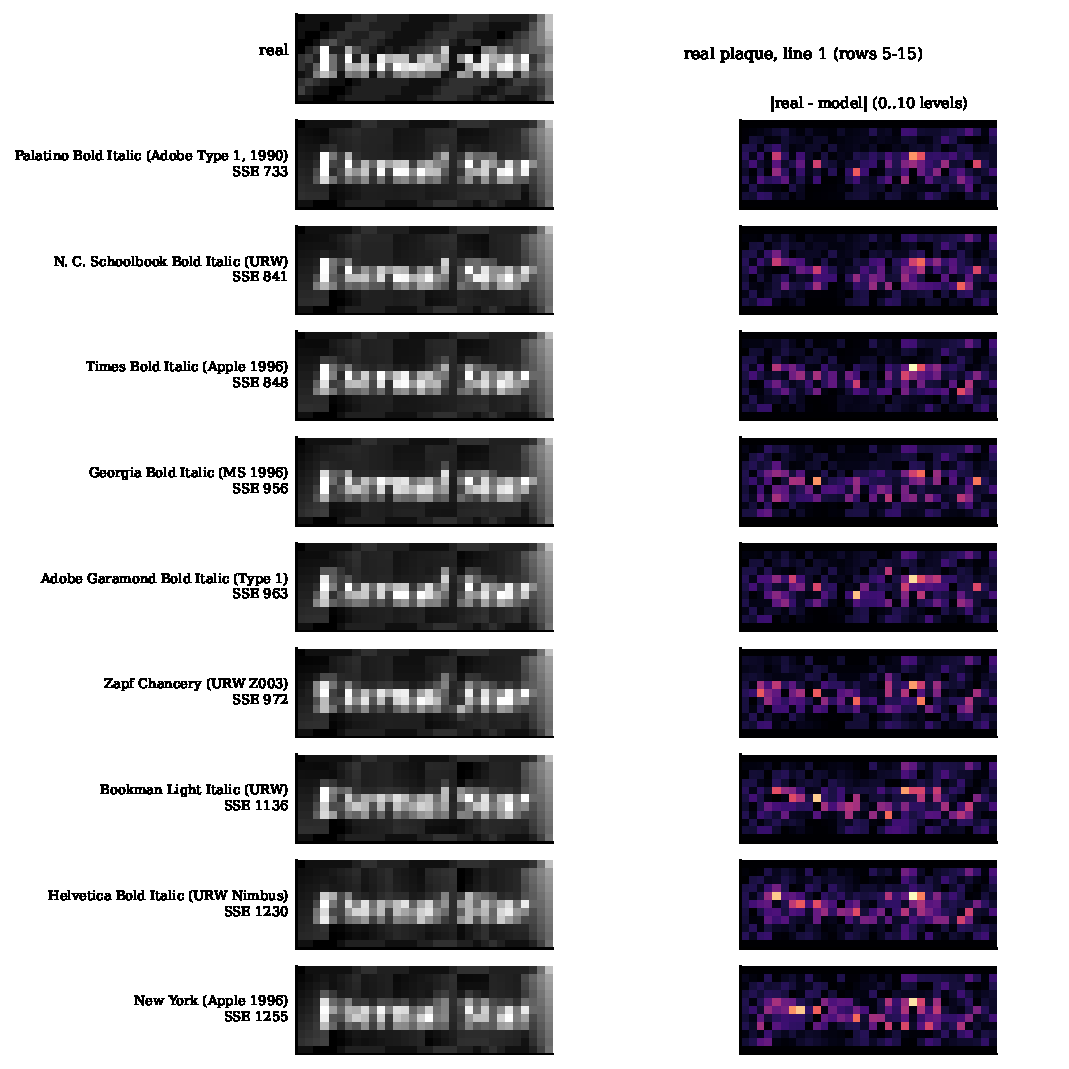
\includegraphics[width=0.95\linewidth]{font_panels.pdf}
\caption{Line~1 as printed by the best recipe of each font family (left) and the absolute difference to the real plaque
(right; 0--10 grey levels).}
\label{fig:fontpanels}
\end{figure}

\paragraph{The in-game font.}
Many players assume the plaque uses \emph{Super Mario 64}'s own dialog font. We tested this directly.
\begin{itemize}
\item \textbf{Setup.} The 71 glyphs and the game's letter widths are extracted from the ROM (US, segment~2, IA4). The
line is typed in the game font and scaled up, either as pixel art (nearest neighbour) or with Photoshop's default
bicubic. It then goes through exactly the same canvas, resize, blur, gamma and position search as every other font.
\item \textbf{Result.} Its best \q{Eternal Star} error is \GameRigid{} on the comparison grid and \GameFull{} with the
full grid (\GameRigidRatio{} times the noise floor), against 757--759 for Palatino Bold Italic. That ranks it
\GameRank{} of \GameOf{} fonts.
\item \textbf{Flexible tournament.} The game font also loses there (\GameFlex{} vs.\ 554).
\item \textbf{Downstream decoding.} With the game font, a dictionary search for the second word does not return
\q{Star} at the top: it was rank 86 in our earlier rounds.
\item \textbf{Why.} The dialog font is a small bitmap font with one-pixel strokes, no serifs and no stroke contrast. The
plaque's letters have the serifs and the thick--thin contrast of an old-style italic.
\item \textbf{Verdict.} The plaque was \emph{not} set in the game's font; it was typeset with a desktop font.
\end{itemize}

\paragraph{Consistency checks.}
\begin{enumerate}
\item \textbf{Two independent Palatinos agree.} The free URW clone (P052) and the genuine Apple 1996 TrueType
Palatino independently converge on the \emph{same} process recipe (\cref{sec:process}).
\item \textbf{Only Palatino decodes cleanly.} When the second word of line~1 or the words of line~2 are searched over
a dictionary, Palatino returns \q{Star} and \q{hope} at rank~1. Times-family fonts return junk strings at the top,
with \q{star} at rank 14--91.
\item \textbf{Weight and style.} Bold Italic and Italic are both close; upright Roman and Bold are clearly worse.
The plaque is italic.
\end{enumerate}

\paragraph{Verdict.} The plaque is typeset in \textbf{Palatino Italic, most likely Bold Italic}, the classic
Hermann Zapf design in its 1990s Mac/PostScript form. Among all Palatino digitisations, Adobe's original 1990 Type~1
file fits best; \cref{sec:adobe} identifies it as the artist's most likely font file.

%======================================================================================================
\section{Reconstructing the process}
\label{sec:process}
Starting from a plain square canvas, we added one designer-plausible global step at a time (\cref{fig:progression}):
\begin{enumerate}
\item \textbf{Non-square artwork.} The art is drawn wider than tall and squeezed into the square texture. The quad
itself is about 1.35:1.
\item \textbf{Word space, light blur and gamma.} The fit chooses $\gamma=1.8$, the classic Macintosh display gamma.
\item \textbf{Whole-pixel advances.} Mac text without fractional widths places every letter on whole pixels.
\end{enumerate}
The final recipe (\cref{tab:recipe}) reaches \SSE~757 (URW) and 759 (Apple), 4.6 times the noise floor. Both fonts
choose the \emph{same} canvas, size, tracking, filter, word space, blur and gamma. Adobe's own 1990 Type~1 file
(first column; \cref{sec:adobe}) prefers slightly larger artwork (192$\times$160, 26\,px) and fits better than both.
The last two rows repeat the comparison against the extracted plain stone of \cref{sec:stone}: the order is unchanged.

\begin{figure}[t]\centering
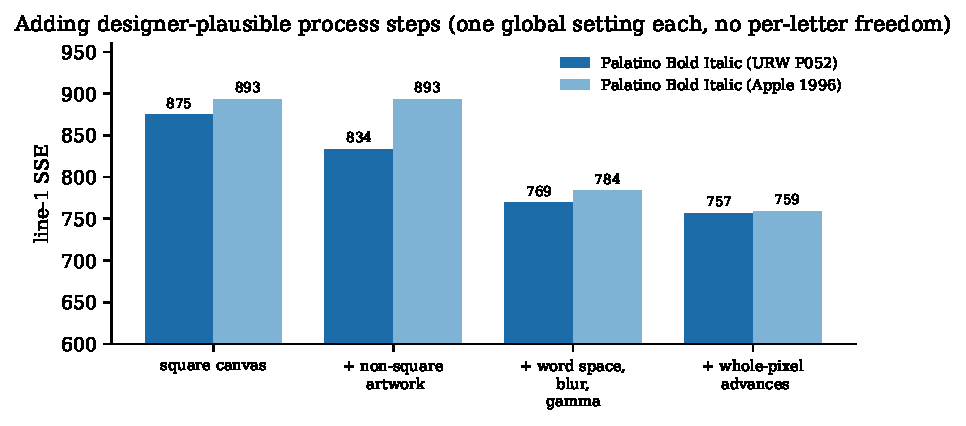
\includegraphics[width=0.9\linewidth]{progression.pdf}
\caption{Each added process step is one global setting, chosen from a short list of options. The error drops from 875
to 757.}
\label{fig:progression}
\end{figure}
\begin{table}[t]\centering\small
\IfFileExists{tables/recipe.tex}{\begin{tabular}{lccc}\toprule
 & Palatino Bold Italic (Adobe Type 1, 1990) & Palatino Bold Italic (URW P052) & Palatino Bold Italic (Apple 1996) \\ \midrule
artwork canvas & 192$\times$160 px & 160$\times$128 px & 160$\times$128 px \\
font size & 26 px & 23 px & 23 px \\
tracking & +2 px & +1 px & +1 px \\
pair kerning & on & off & on \\
advances & whole pixels per glyph & whole pixels per glyph & whole pixels per glyph \\
word space & +0.0 texture px & -0.5 texture px & -0.5 texture px \\
resize filter & bilinear & bilinear & bilinear \\
blur after resize & $\sigma=0.30$ px & $\sigma=0.45$ px & $\sigma=0.45$ px \\
gamma & 1.4 & 1.8 & 1.8 \\
line-1 SSE (stone planes) & 731.3 & 756.9 & 759.2 \\
SSE / noise floor & 4.41 & 4.57 & 4.58 \\
same recipe, fixed stone & 788.7 & 823.8 & 811.4 \\
best recipe, fixed stone & 788.7 & 814.0 & 811.4 \\
\bottomrule\end{tabular}
}{}
\caption{The reconstructed designer recipe for line~1: Adobe's 1990 file and the two independent Palatinos.}
\label{tab:recipe}
\end{table}

\paragraph{What is still missing?}
A flexible model that may shift each letter horizontally reaches 548. With the per-letter shifts switched off, the same
flexible model is \emph{worse} than our rigid recipe (\cref{fig:ablation}). The remaining gap is therefore pure letter
spacing:
\begin{itemize}
\item \q{r n a l} sit about 0.3\,px further right than these fonts place them;
\item \q{Star} sits about 0.35\,px to the left, which a narrower word space explains.
\end{itemize}
Eleven extra parameters on pure noise would buy about 6 \SSE, not the 200 observed. The true 1996 spacing therefore
genuinely differs slightly, through hinting by an unknown rasteriser or hand kerning. This affects neither the font
family nor the words.

\begin{figure}[t]\centering
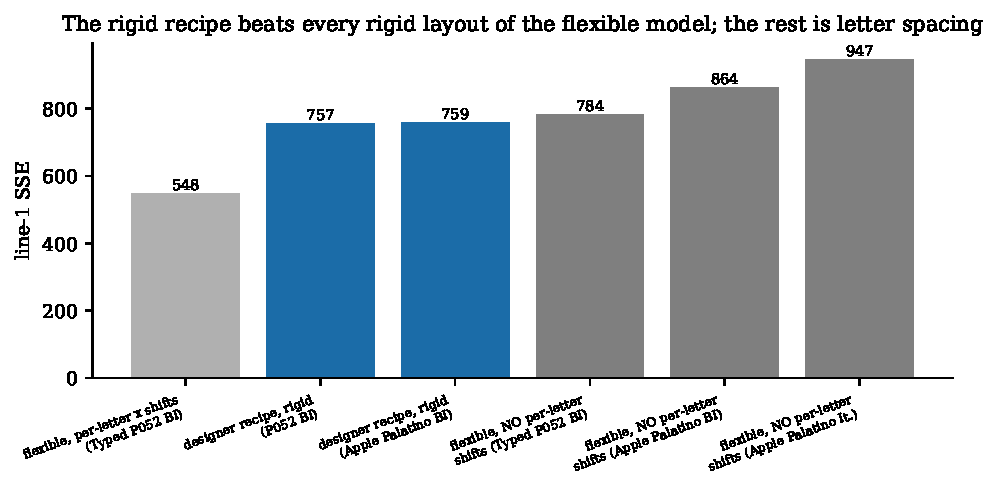
\includegraphics[width=0.95\linewidth]{ablation.pdf}
\caption{Ablation. The rigid recipe (blue) beats every rigid layout of the flexible model (grey); only free per-letter
shifts do better.}
\label{fig:ablation}
\end{figure}

%======================================================================================================
\section{Line 1: \q{Eternal Star}}
\label{sec:line1}
\paragraph{\q{Eternal}.}
The first word is robust across every font, process and test. Its letters E, t and l are individually confirmed by
local fits.

\paragraph{The second word, with every setting frozen.}
We froze the complete recipe (font, canvas, size, tracking, filter, blur, gamma and position) and rendered
\q{Eternal\,\_\_\_} for each of 27{,}122 dictionary words. Only the word space (4 values) and the ink level remained free.
\begin{itemize}
\item \q{Star} is \textbf{rank~1 in both fonts} (\cref{fig:word2}).
\item The runners-up (Stat, Sent, Seat) share its shape: S, a tall letter, two small letters.
\end{itemize}

\paragraph{Fairness.}
The recipe was tuned on \q{Star}, so we re-ran the \emph{entire} recipe search separately for each rival
(\cref{fig:rivals}).
\begin{itemize}
\item \q{Star}/\q{star} still beat Stat, Sent, Slot and Seat.
\item On line~1 alone, upper- and lower-case \q{s} are tied: 757 vs.\ 755 (URW) and 759 vs.\ 765 (Apple).
\item \textbf{Joint two-line test.} One process must explain both lines. For each spelling we took its 100 best line-1
recipes and scored line~2 (\q{We hope so}) under each of them, then compared the best totals.
  \begin{itemize}
  \item Genuine Apple font: \q{Eternal Star} \JointAUp{} vs.\ \q{Eternal star} \JointALo, so the capital S is ahead.
  \item URW clone: \JointUUp{} vs.\ \JointULo, so the lower-case s is ahead.
  \end{itemize}
The two fonts disagree, so \textbf{the case of the s remains undecided}. We write \q{Eternal Star}, but the pixels do
not settle it.
\end{itemize}

\begin{figure}[t]\centering
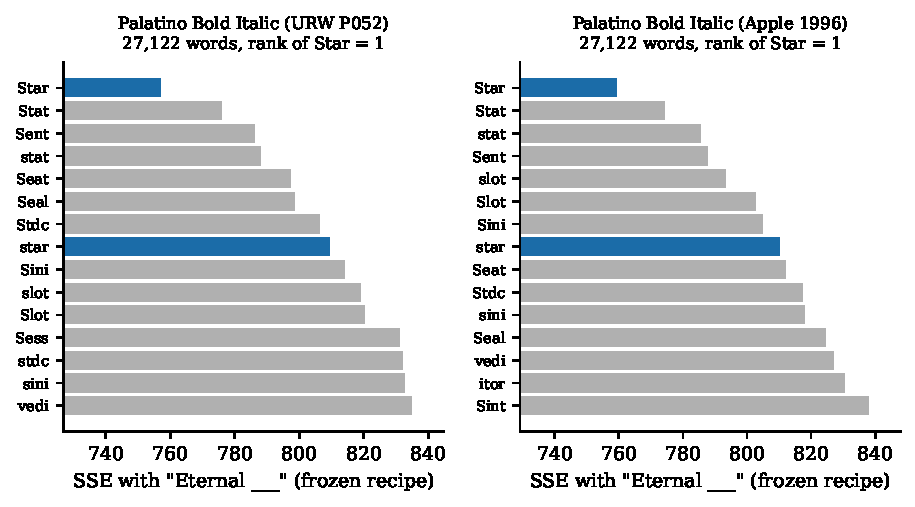
\includegraphics[width=0.95\linewidth]{word2.pdf}
\caption{The second word of line~1 under the frozen recipe: top~15 of 27{,}122 words.}
\label{fig:word2}
\end{figure}
\begin{figure}[t]\centering
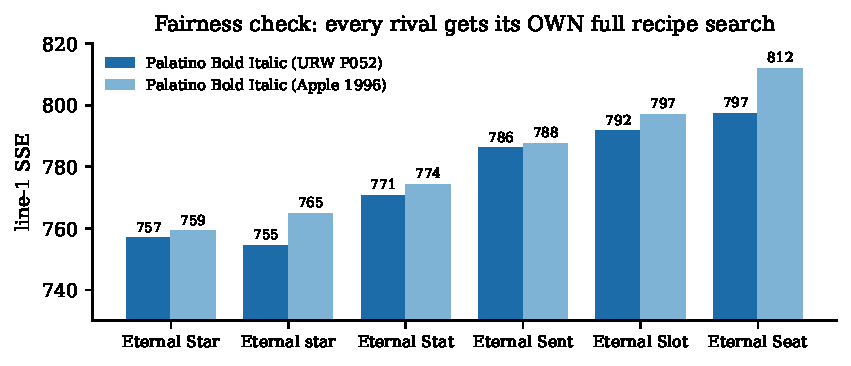
\includegraphics[width=0.8\linewidth]{rivals.pdf}
\caption{Every rival second word gets its own complete recipe search.}
\label{fig:rivals}
\end{figure}

%======================================================================================================
\section{Line 2: \q{We hope so}}
\label{sec:line2}
\paragraph{Locked process.}
We assume the designer set line~2 in the same document. It therefore shares the face, canvas, tracking, advance mode,
filter, blur, gamma and \emph{ink level} of line~1. This removes the contrast freedom that let nonsense win in
earlier attempts. Only the size, the baseline, the start position and the word space are free.

\paragraph{Fast exact-enough search.}
Every glyph at every canvas position is pre-rendered through the process as a small \q{tile}, and a string is a sum of
tiles. A K-best dynamic programme then finds the best \emph{word sequences}: any number of words, any start position,
over a 17.7k-word English vocabulary. It runs for every size (13--20\,px), baseline and word space. The top 3{,}000
phrases are re-rendered exactly.

\paragraph{What comes out unprompted.}
\begin{itemize}
\item \textbf{Size and spacing:} 17\,px, with exactly line~1's narrower word space.
\item \textbf{Centring:} the line sits under line~1 (ink centre column 15.0 vs.\ 15.5), consistent with centred text.
\item \textbf{Words:} \DPHopeShare{} of the top 60 sequences contain the word \q{hope}, and almost all begin with a
W-word (\cref{fig:dp}).
\end{itemize}

\begin{figure}[t]\centering
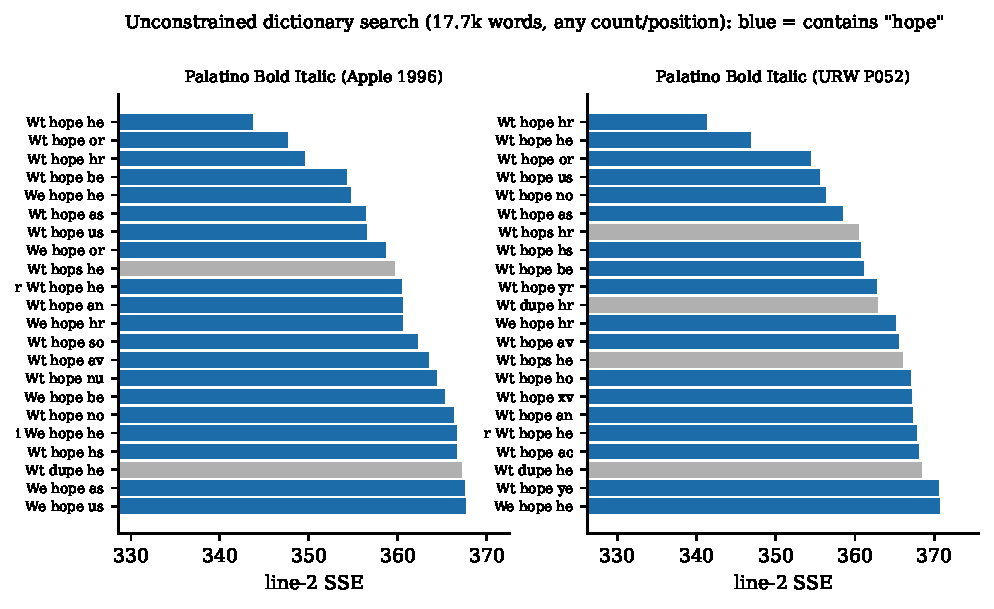
\includegraphics[width=0.98\linewidth]{line2_dp.pdf}
\caption{Unconstrained dictionary search for line~2. Without being told anything, \q{hope} appears in nearly every top
sequence (blue).}
\label{fig:dp}
\end{figure}

\paragraph{Exhaustive slot tests (\cref{fig:slots}).}
\begin{itemize}
\item \textbf{Middle word.} In \q{We\,\_\_\_\,so}, \q{hope} is \textbf{rank 1 of 12{,}556 words in both fonts}, 16--19
\SSE{} ahead of \q{hops}; everything else is more than 24 behind.
\item \textbf{First word.} Among all 157k strings of one to three letters, the pixels want a capital W followed by one
small letter. \q{We} is the best English word, ahead of \q{Me} and \q{He}.
\item \textbf{Ending.} The ending is two x-height letters. \q{he, or, us, as, be, no, an, so} lie within about 20 \SSE{}
of each other.
\end{itemize}

\begin{figure}[t]\centering
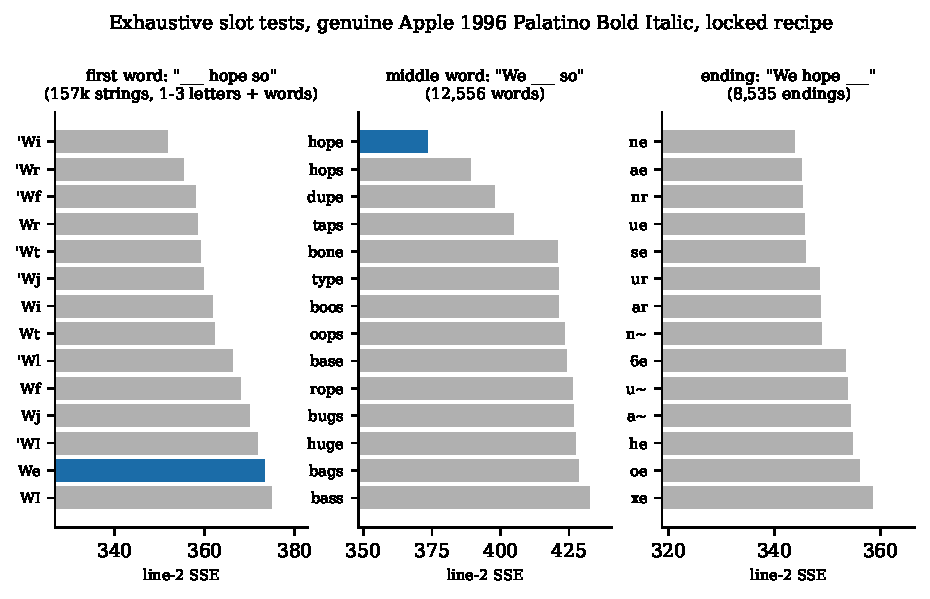
\includegraphics[width=0.98\linewidth]{line2_slots.pdf}
\caption{Slot tests with the genuine Apple 1996 Palatino Bold Italic: first word, middle word and ending.}
\label{fig:slots}
\end{figure}
\begin{table}[t]\centering\small
\IfFileExists{tables/line2_variants.tex}{\begin{tabular}{lrrrl}\toprule
 line 2 & Apple & URW & mean & complete sentence? \\ \midrule
``We hope he'' & 355 & 371 & 363 & no \\
``We hope or'' & 359 & 378 & 368 & no \\
``We hope us'' & 368 & 379 & 373 & no \\
``We hope no'' & 377 & 380 & 379 & no \\
``We hope so'' & 373 & 389 & 381 & yes \\
``Me hope so'' & 392 & 385 & 389 & no \\
``We hope so.'' & 386 & 392 & 389 & yes \\
``We hope on'' & 382 & 408 & 395 & yes \\
``We hope to'' & 397 & 416 & 406 & no \\
``We hope so!'' & 411 & 407 & 409 & yes \\
``We hope is'' & 404 & 421 & 412 & no \\
``My hope so'' & 435 & 410 & 423 & no \\
``He hope so'' & 441 & 429 & 435 & no \\
``We hope for'' & 460 & 434 & 447 & no \\
``No hope so'' & 461 & 464 & 463 & yes \\
``My hope is'' & 481 & 459 & 470 & yes \\
``We hope it'' & 467 & 477 & 472 & no \\
``my hope is'' & 489 & 475 & 482 & yes \\
``We hope all'' & 510 & 461 & 485 & no \\
``We Hope So'' & 523 & 481 & 502 & yes \\
``We hope one'' & 514 & 492 & 503 & no \\
``We hope too'' & 532 & 484 & 508 & no \\
``'Tis hope so'' & 554 & 471 & 512 & no \\
``To hope is'' & 523 & 538 & 530 & yes \\
``We hope for it'' & 550 & 524 & 537 & yes \\
``We hope \textasciitilde{}'' & 522 & 585 & 553 & no \\
``We hope you'' & 564 & 587 & 576 & no \\
``We hope to see'' & 647 & 628 & 638 & yes \\
``We hope'' & 682 & 696 & 689 & no \\
``We hope!'' & 716 & 720 & 718 & no \\
``He hopes so'' & 742 & 743 & 742 & yes \\
``I hope so'' & 1047 & 1024 & 1035 & yes \\
\bottomrule\end{tabular}
}{}
\caption{Exact line-2 errors (whole band) of the main variants in both fonts, and whether each forms a complete sentence.
Line-2 noise floor 165.7; stone only (no text) \LineTwoStone.}
\label{tab:variants}
\end{table}

\paragraph{The ending under line~1's typesetting.}
\Cref{tab:variants} lists the main variants. The simulations in \cref{sec:calib} show that two-letter endings within
about 20 \SSE{} cannot be separated by the pixels: a planted \q{We hope so} was decoded as \q{We hope an}. Of the
pixel-compatible endings, \q{so} is the only one that forms a complete sentence. Once line~2's own typesetting is
calibrated (\cref{sec:hope}), \q{so} also becomes the best-fitting real ending.

Several alternatives are clearly worse:
\begin{itemize}
\item a Zapf Dingbats star, punctuation-only endings and Japanese-style \q{\textasciitilde}
endings;
\item \q{We hope you};
\item Title Case \q{We Hope So};
\item no ending at all, which scores 682.
\end{itemize}

\begin{figure}[t]\centering
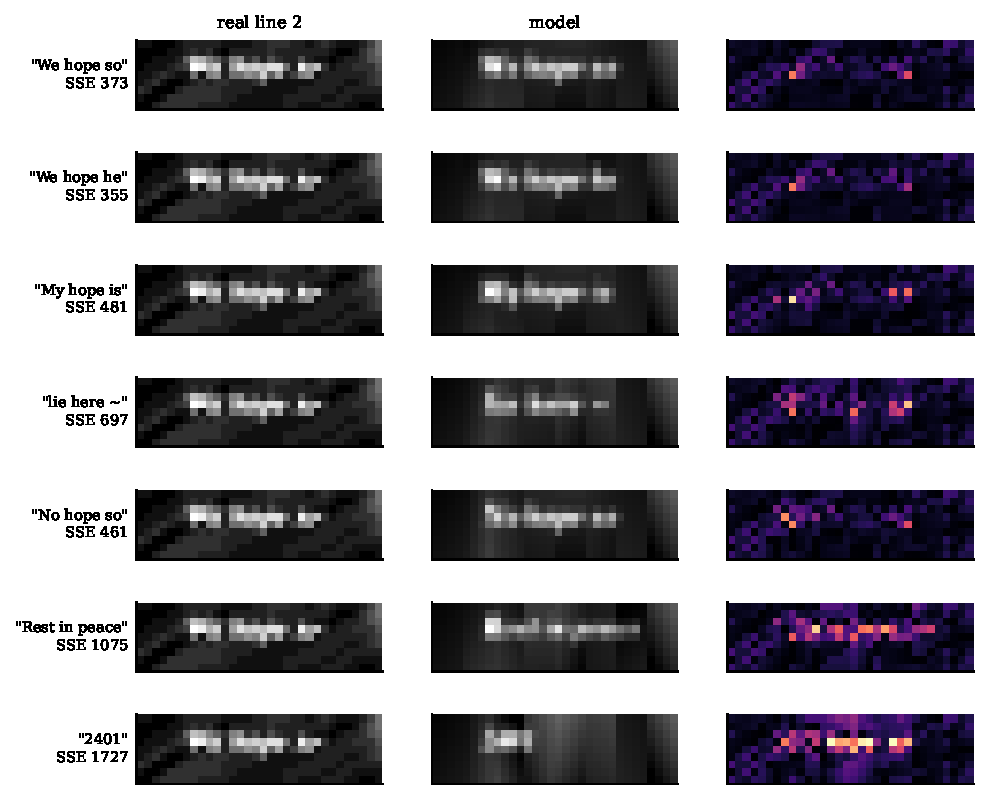
\includegraphics[width=0.9\linewidth]{line2_panels.pdf}
\caption{Line~2 band: real pixels, model and difference for several readings.}
\label{fig:l2panels}
\end{figure}

\paragraph{Descenders.}
Row~20 lies just below the line-2 baseline. It is significantly brighter than the stone below it in \emph{one} place
only: column~\DescCol{} (+\DescVal{} levels; clean-stone s.d.\ \StoneSD), which is exactly where the \q{p} of \q{hope}
falls (\cref{fig:descender}). A reading with two descenders, such as \q{My hope is}, predicts a second descender under
the \q{y} that the texture does not show.

\begin{figure}[t]\centering
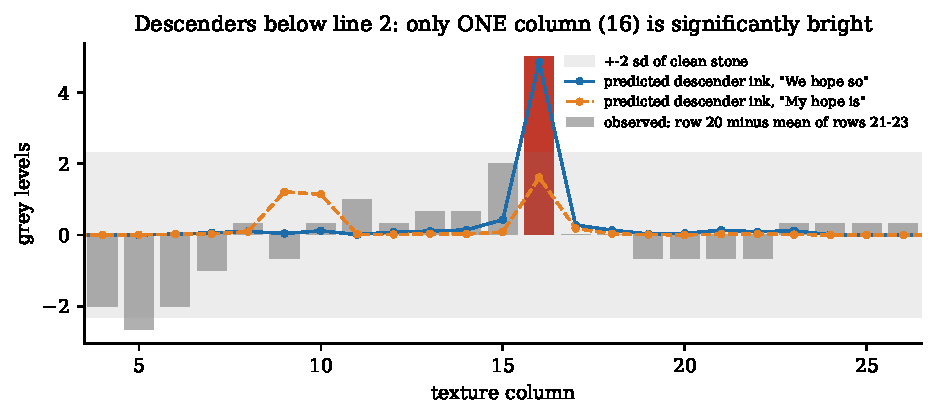
\includegraphics[width=0.95\linewidth]{descender.pdf}
\caption{Descender evidence. Bars: brightness of row~20 relative to the stone below. Lines: descender ink predicted by
\q{We hope so} and \q{My hope is}.}
\label{fig:descender}
\end{figure}


\subsection*{Close-up: candidates for \q{We} and for \q{so}}
These are the two least certain words, so we isolated them. In each test the rest of the line is held fixed: either
\q{\_\_\_\ hope so} or \q{We hope \_\_\_}. Each candidate is rendered as a whole line with the locked recipe, but scored
only on the stone blocks that contain the word in question:
\begin{itemize}
\item first word: texture columns 0--11;
\item ending: texture columns 20--31.
\end{itemize}
Because each region is scored on its own pixels, the comparison is not diluted by the rest of the line. The best
non-word strings found by the exhaustive search are shown for reference (\cref{fig:candbars,fig:candfirst,fig:candend}).

\paragraph{First word.}
\begin{itemize}
\item \textbf{What the pixels want.} A wide capital with a double-bowl or double-V top, followed by small letters.
The non-words \q{Wi}, \q{Wr} and \q{Wt} sit at the very top in both fonts.
\item \textbf{Best real words.} \q{We'll}, \q{We} and \q{By} are a tight group on their own region: \q{We} scores
\LocFAWe{} (Apple) and \LocFBWe{} (URW), and \q{By} \LocFABy{} (Apple).
\item \textbf{Clearly worse in both fonts:} \q{Me}, \q{He}, \q{My}, \q{No} and \q{Be}.
\item \textbf{Whole-line test.} A local fit is not enough, because the first word's width fixes where \q{hope so} must
sit. On the whole line, \q{We'll} and \q{By} push \q{hope so} out of place and fail (\cref{sec:hope}); only \q{We}
remains.
\end{itemize}

\paragraph{Ending.}
\begin{itemize}
\item \textbf{Shape.} The ending is two x-height letters, with a bright stroke at the start and a rounded second
letter. The best non-words (\q{ne}, \q{nr}, \q{ae}) show exactly this.
\item \textbf{Ranking of real endings.} In both fonts: \q{he} (\LocEAHe\,/\,\LocEBHe), then \q{or}, \q{us}, \q{as},
\q{be}, \q{no} (the order varies slightly between fonts), then \q{so} (\LocEASo\,/\,\LocEBSo).
\item \textbf{Clearly worse:} \q{to}, \q{for} and \q{is}. Their ascenders and the long \q{for} add ink where the
texture has none.
\item \textbf{What can be resolved.} The spread from \q{he} to \q{so} is about 20 local \SSE. The simulations
(\cref{sec:calib}) show that differences of this size between two-letter endings cannot be resolved: a planted
\q{We hope so} came back as \q{We hope an}.
\end{itemize}

\paragraph{Variants.}
\Cref{tab:variants} and \cref{fig:variants,fig:variantpanels} compare whole-line variants.
\begin{itemize}
\item The four best-fitting lines are \q{We hope he}, \q{\ldots or}, \q{\ldots us} and \q{\ldots no}. None of them is a
complete sentence.
\item \textbf{The best-fitting \emph{complete} sentence is \q{We hope so}}, in both fonts. It is followed by \q{We hope
so.} and \q{We hope on}.
\item \q{We hope to}, \q{We hope is}, \q{We hope for}, \q{My hope is}, \q{He hopes so} and \q{I hope so} are clearly
worse.
\end{itemize}

\begin{figure}[p]\centering
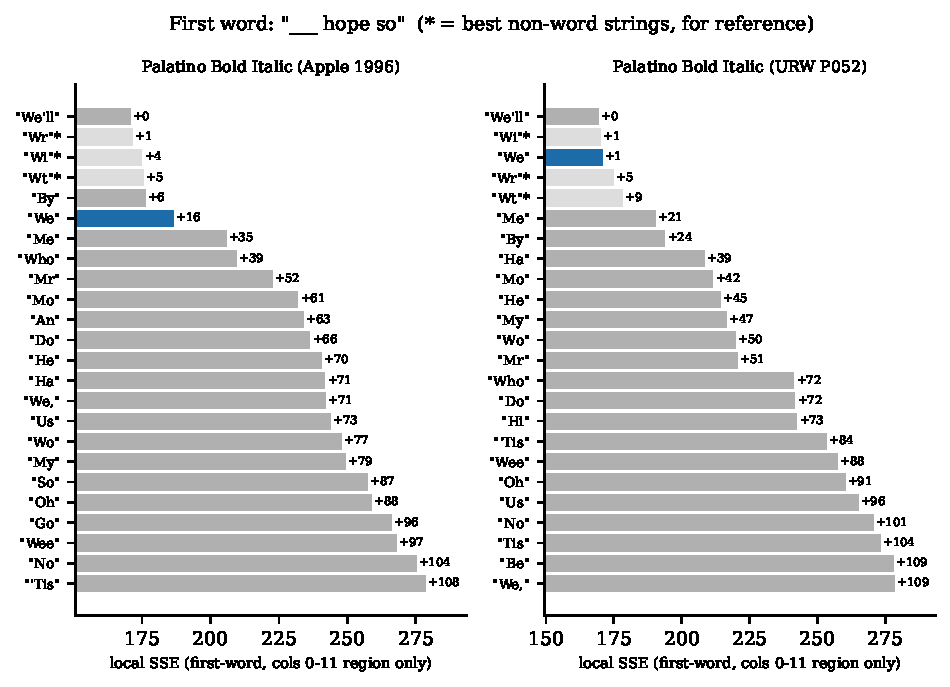
\includegraphics[width=0.95\linewidth]{cand_first_bars.pdf}\\[2mm]
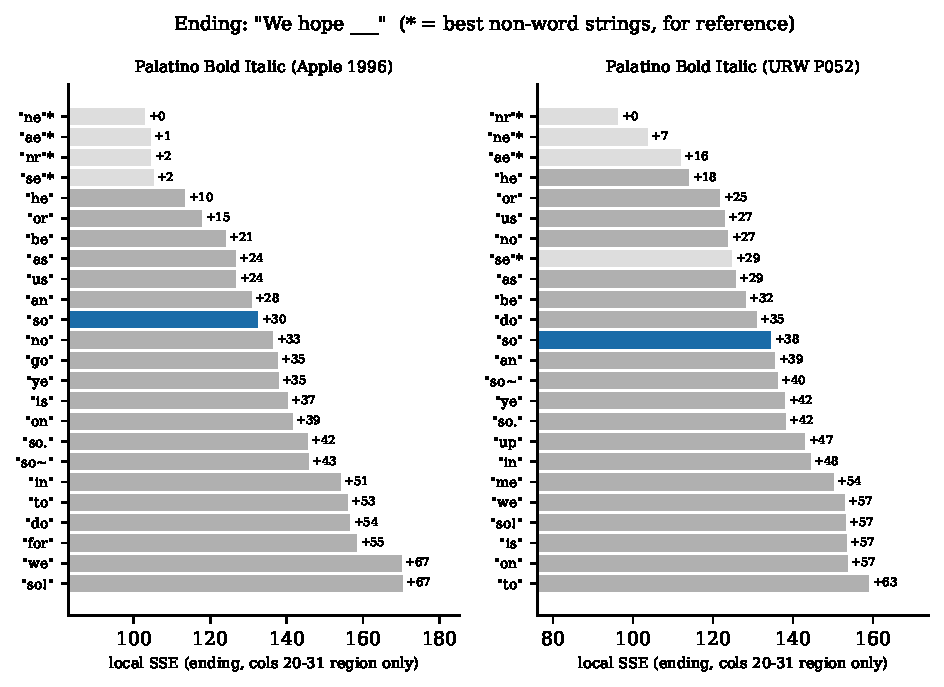
\includegraphics[width=0.95\linewidth]{cand_end_bars.pdf}
\caption{Local errors of first-word candidates (top) and ending candidates (bottom) in both fonts. Blue: our reading.
Light grey with *: best non-word strings, for reference.}
\label{fig:candbars}
\end{figure}
\begin{figure}[p]\centering
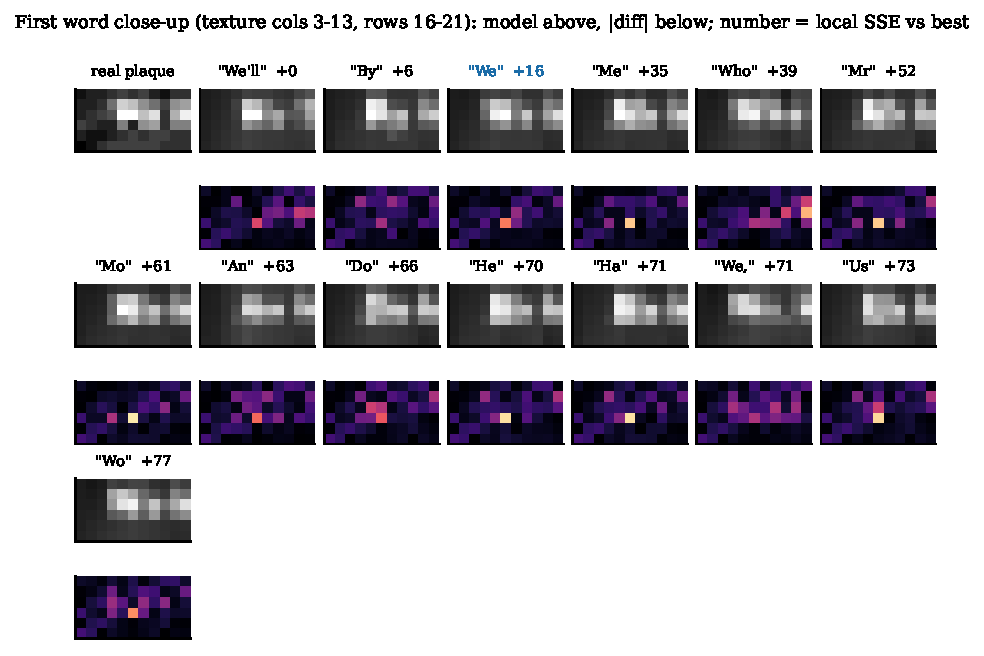
\includegraphics[width=\linewidth]{cand_first_crops.pdf}
\caption{Close-up of the first word (Apple Palatino). For each candidate, the model of the zoomed region is shown
above and the absolute difference to the real plaque below. The number is the local \SSE{} relative to the best
candidate.}
\label{fig:candfirst}
\end{figure}
\begin{figure}[p]\centering
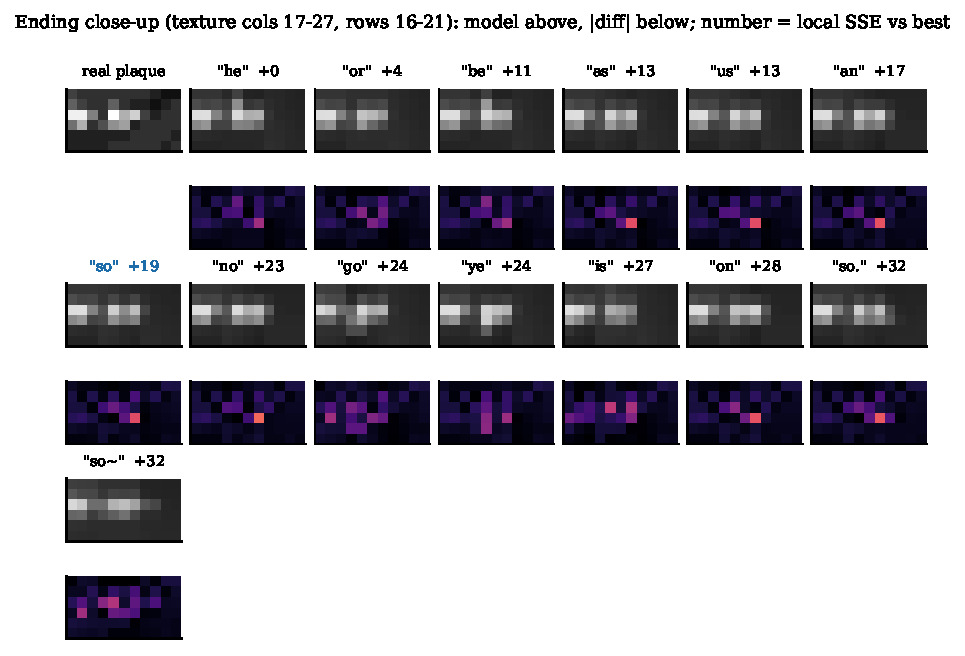
\includegraphics[width=\linewidth]{cand_end_crops.pdf}
\caption{Close-up of the ending (Apple Palatino), laid out as in \cref{fig:candfirst}.}
\label{fig:candend}
\end{figure}
\begin{figure}[p]\centering
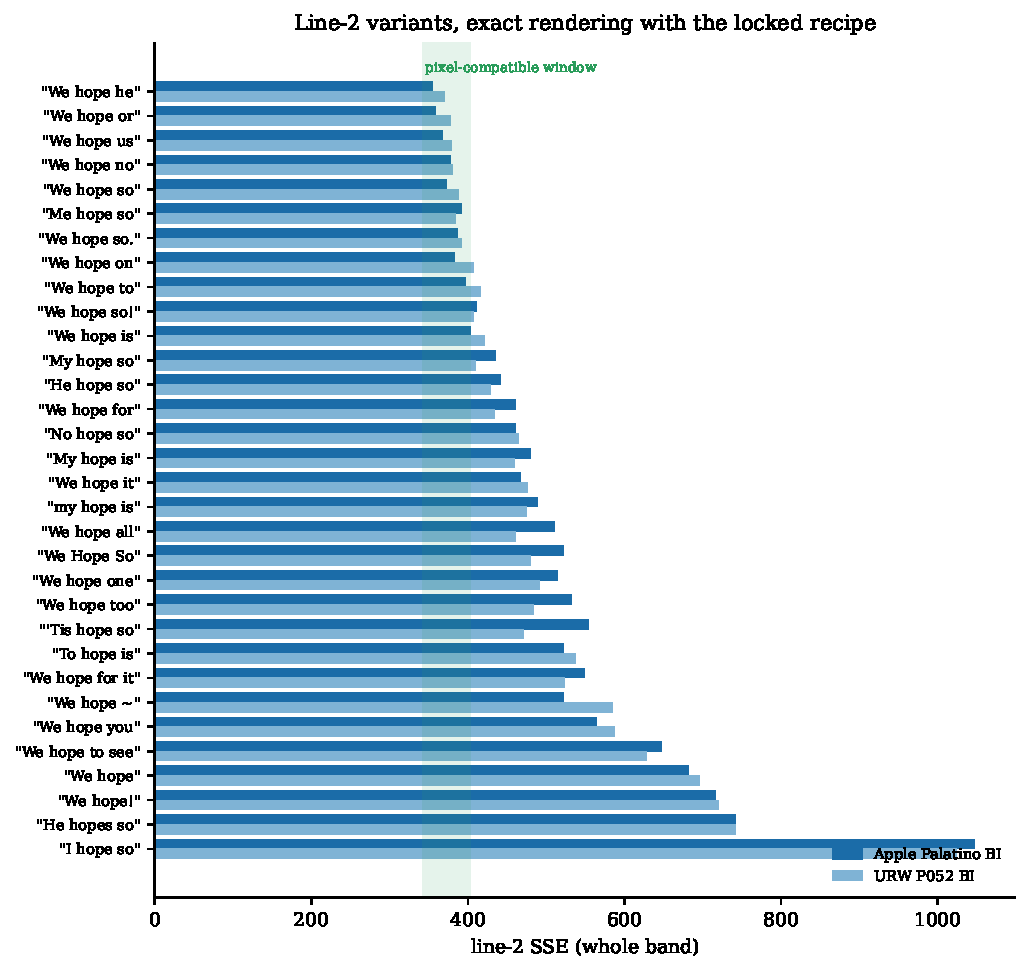
\includegraphics[width=0.95\linewidth]{variants.pdf}
\caption{Whole-line variants in both fonts. The green band is the pixel-compatible window (\cref{sec:calib}).}
\label{fig:variants}
\end{figure}
\begin{figure}[p]\centering
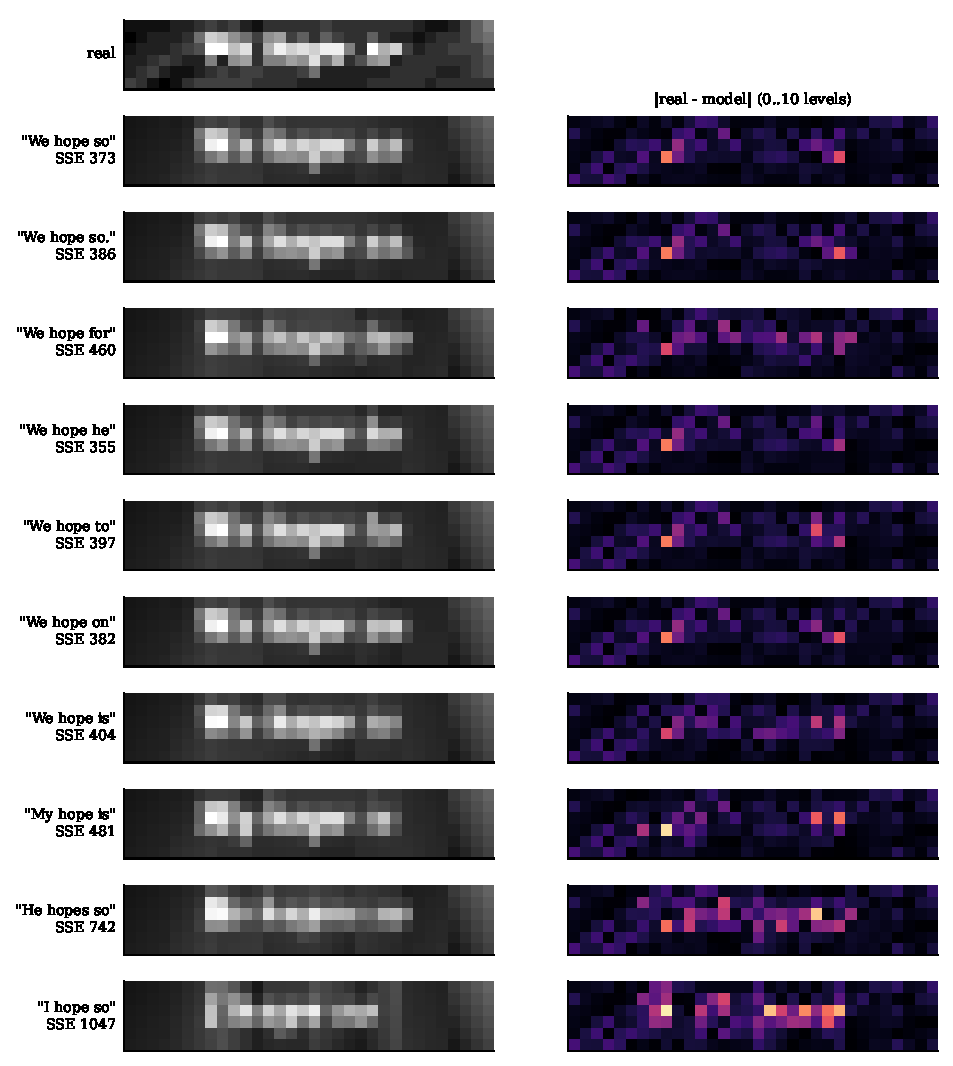
\includegraphics[width=0.92\linewidth]{variant_panels.pdf}
\caption{Line~2 for the main variants: model (left) and absolute difference to the real plaque (right).}
\label{fig:variantpanels}
\end{figure}


\paragraph{Other first words and other sentences.}
We also tried alternatives suggested by the first-word close-up, and sentences that would make good sense on such a
plaque, including quirky Japanese-English phrasings a 1996 Japanese team might have written.
\begin{itemize}
\item \textbf{Seeded search.} The global dictionary search was seeded with the first words We, By, Be, Me, My, He (and
variants), with everything after them free. A further 91{,}884-phrase set combined these first words with about 90
middle words and 40 endings, in sentence and Title case.
\item \textbf{\q{hope} survives every first word.} The best line for each first word is: \q{\AltPhAWe} (\AltAWe),
\q{\AltPhAMe} (\AltAMe), \q{\AltPhAHe} (\AltAHe), \q{\AltPhAMy} (\AltAMy), \q{\AltPhABy} (\AltABy) and \q{\AltPhABe}
(\AltABe), all in Apple Palatino.
\item \textbf{\q{We} gives the best fit by a wide margin.} \q{By} matches its own region well, but its width pushes
\q{hope} out of place.
\item \textbf{Other sentences are far outside the pixel-compatible window} (\cref{tab:alternatives},
\cref{fig:altpanels}): \q{Be with us} and its variants, \q{By your side}, \q{We love you}, \q{Be happy}, \q{We pray so}
and \q{We hope you}. None of them reproduces the tall-first-letter, mid-word-descender shape of the middle word.
\end{itemize}

\begin{table}[t]\centering\small
\IfFileExists{tables/line2_alternatives.tex}{\begin{tabular}{lrrr}\toprule
 line 2 & Apple & URW & mean \\ \midrule
``We hope he'' & 355 & 371 & 363 \\
``We hope so'' & 373 & 396 & 385 \\
``By hope so'' & 434 & 409 & 421 \\
``Be hope so'' & 492 & 493 & 493 \\
``We pray so'' & 550 & 537 & 543 \\
``We hope you'' & 552 & 587 & 569 \\
``We wish so'' & 675 & 555 & 615 \\
``By my side'' & 653 & 654 & 654 \\
``We hope it so'' & 695 & 662 & 679 \\
``Be my star'' & 681 & 685 & 683 \\
``Be with us'' & 730 & 666 & 698 \\
``Be with me'' & 724 & 675 & 699 \\
``Be with us\textasciitilde{}'' & 731 & 669 & 700 \\
``Be happy so'' & 705 & 726 & 716 \\
``Be with us!'' & 752 & 689 & 720 \\
``Be happy'' & 730 & 720 & 725 \\
``We love you'' & 708 & 751 & 729 \\
``Be With Us'' & 780 & 736 & 758 \\
``By your side'' & 760 & 766 & 763 \\
``We are hope'' & 752 & 793 & 772 \\
``Be my hope'' & 794 & 771 & 783 \\
``We keep hope'' & 764 & 811 & 788 \\
``Be here now'' & 837 & 796 & 817 \\
``Be at peace'' & 873 & 798 & 835 \\
``Be with you'' & 867 & 858 & 863 \\
``Be our hope'' & 886 & 861 & 873 \\
``Be here'' & 889 & 865 & 877 \\
``Wish so'' & 906 & 926 & 916 \\
``Be safe'' & 927 & 916 & 921 \\
``We be ok'' & 933 & 924 & 928 \\
``Hope so'' & 1000 & 947 & 973 \\
``Be well'' & 1062 & 1053 & 1057 \\
``Be ok'' & 1297 & 1264 & 1280 \\
\bottomrule\end{tabular}
}{}
\caption{Alternative sentences for line~2 (exact, locked recipe; lower is better).}
\label{tab:alternatives}
\end{table}
\begin{figure}[t]\centering
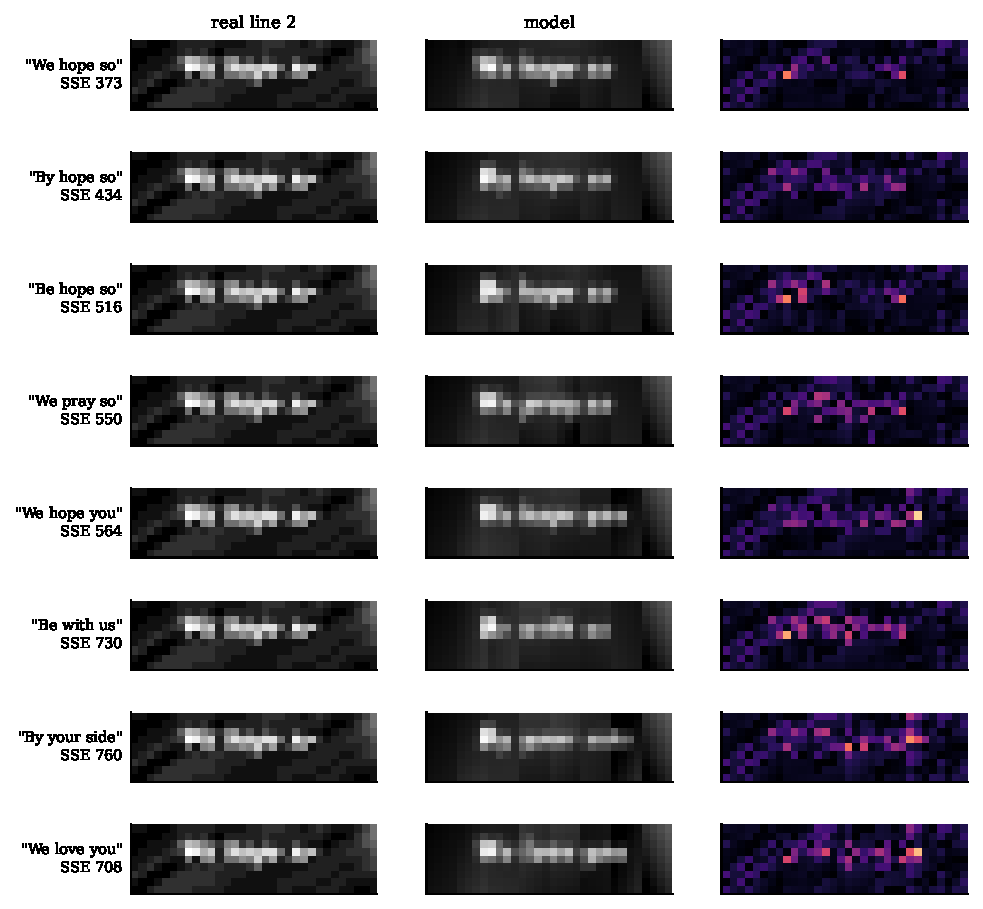
\includegraphics[width=0.9\linewidth]{alt_panels.pdf}
\caption{Line~2 for alternative sentences: model (middle) and absolute difference (right) next to the real plaque (left).}
\label{fig:altpanels}
\end{figure}


%======================================================================================================
\section{Working backwards from \q{hope}}
\label{sec:hope}
For line~1 we assumed the text and solved for the process. We can do the same for line~2, using its most certain word.

\paragraph{What may differ between the lines.}
Canvas, resize filter, blur, gamma and ink colour are \emph{shared}: both lines sit in one image, which is resized once.
Each typed line may still have its own size, tracking, kerning, advance mode and even style. In
\cref{sec:line2} those were copied from line~1.

\paragraph{Fitting line 2's typesetting on \q{hope} alone.}
We render only the word \q{hope} and score it only on its own pixels: the stone blocks covering texture columns
12--19. The search covers:
\begin{itemize}
\item four faces: Palatino Bold Italic and Italic, Apple and URW;
\item sizes 13--21\,px and tracking $-1$ to $+3$;
\item kerning on/off and two advance modes;
\item all positions.
\end{itemize}
Both Bold Italic faces fit equally well (\HopeUFit{} and \HopeAFit), at \textbf{\HopeUSize\,px, tracking
\HopeUTrack{} (line~1: $+1$), whole-pixel advances and no kerning} (\cref{fig:hopefit}). The Italic (non-bold) faces
fit worse.

\begin{figure}[t]\centering
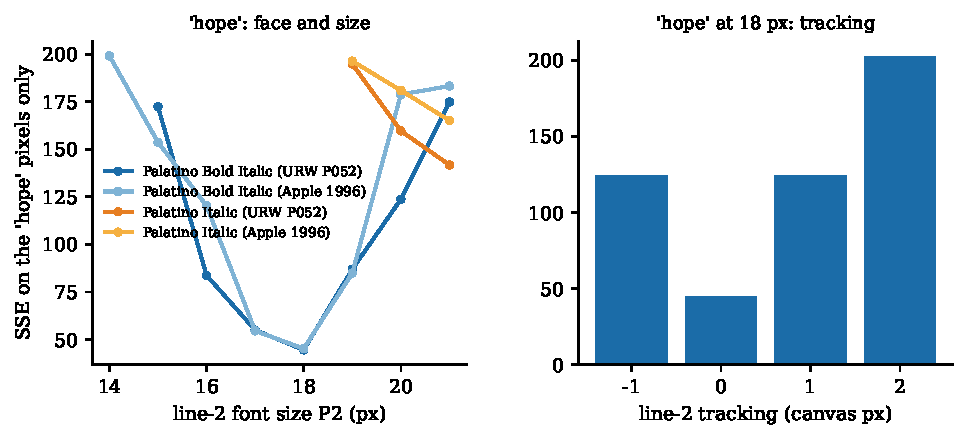
\includegraphics[width=0.95\linewidth]{hopefit.pdf}
\caption{Line-2 typesetting fitted on the four letters of \q{hope} only. Left: error vs.\ font size for four faces.
Right: error vs.\ tracking at the best size.}
\label{fig:hopefit}
\end{figure}

\paragraph{Then judging \q{We} and \q{so} on their own pixels.}
This is a held-out test. The typesetting was calibrated on columns 12--19 only, and the first word and the ending are
then scored on \emph{different} pixels: columns 0--11 and 20--31 (\cref{fig:hopebars,fig:hopecrops}).
\begin{itemize}
\item \textbf{First word (URW line~2).} \q{We} is the best real word (\HopeUFWe). It is ahead of \q{Me} (\HopeUFMe);
\q{By} drops out of contention. Only the non-word \q{Wr} is lower (\HopeUFWr).
\item \textbf{First word (Apple line~2).} The W-forms lead again.
\item \textbf{\q{We'll}.} With the calibrated setting, \q{We'll} matches its own region best of all, because its extra
strokes resemble a faint mark near column~9. On the whole line, however, \q{We'll hope so} scores 642 (URW), against 329
for \q{We hope so}. The wider word pushes \q{hope so} out of place. \q{We'd}, \q{Well}, \q{Will} and \q{We will} fail
in the same way (544--1000). \q{By} shows the same effect, so a good local fit alone is not enough.
\item \textbf{Ending.} \textbf{\q{so} becomes the best real ending in both faces}: \HopeUESo{} vs.\ \q{or} \HopeUEOr,
\q{us} \HopeUEUs, \q{he} \HopeUEHe{} (URW); \HopeAESo{} vs.\ \q{as}, \q{or} \HopeAEOr, \q{us} \HopeAEUs{} (Apple).
Only non-words such as \q{nr} or \q{se} are lower.
\item \textbf{Whole line (URW).} \q{We hope so} becomes the best of all variants (\HopeUVWeHopeSo), ahead of
\q{We hope or} (\HopeUVWeHopeOr), \q{We hope us} (\HopeUVWeHopeUs) and \q{We hope he} (\HopeUVWeHopeHe). It is also the
best line-2 error of the whole study (\cref{fig:hopevariants}).
\end{itemize}

\paragraph{The unconstrained search now finds the sentence on its own.}
We repeated the global dictionary search under the calibrated setting: 17.7k words, any number of words, any position,
no hints (\cref{fig:hopedp}). The best strings are now \q{We hops So}, \q{Wt hope so} and \textbf{\q{We hope so}}
(rank~\HopeDPURankLc, \HopeDPUSseLc; URW). With Apple Palatino the top is \q{We hops So} with \q{We hope So} at
rank~\HopeDPARankUc.
\begin{itemize}
\item Without any guidance, the search now produces \emph{We} at the start and \emph{so} at the end. Under line~1's
typesetting it had preferred \q{he}/\q{hr} endings.
\item The only rival for the middle word is \q{hops}, which differs from \q{hope} by one small letter. That is at the
limit of resolution; \q{hope} is the English choice.
\item Upper- or lower-case \q{so} cannot be distinguished.
\end{itemize}

\paragraph{Why this matters.}
Calibrating the typesetting on one word made the other two words come out without being told. This is the same
self-consistency that identified \q{Eternal Star}: one process and one font explain the whole line, and they predict
\q{We} and \q{so} on pixels that were not used to fit them.

\begin{figure}[p]\centering
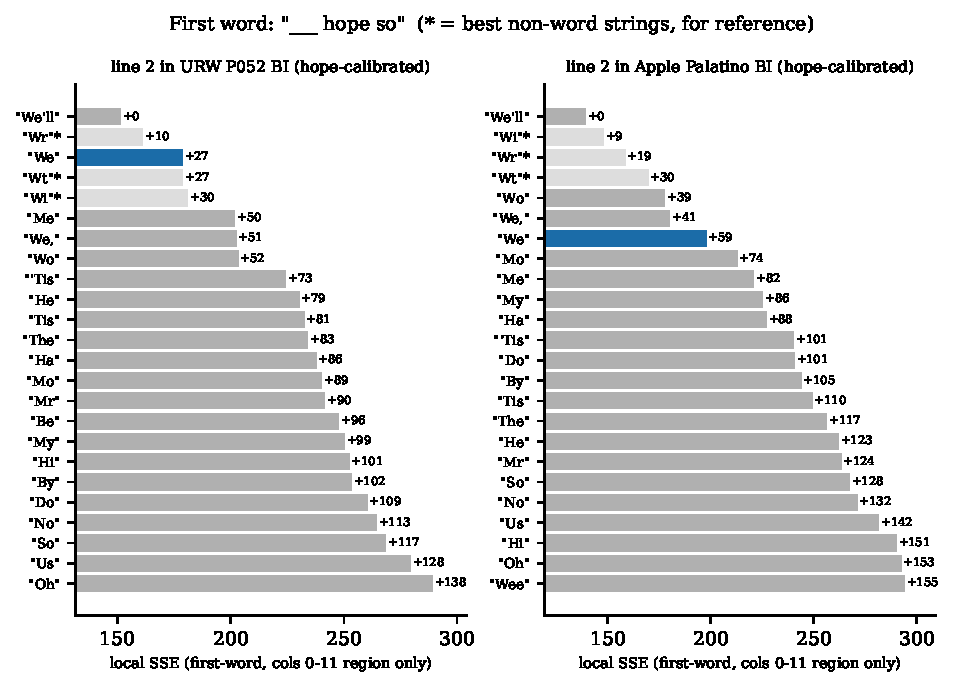
\includegraphics[width=0.95\linewidth]{hope_first_bars.pdf}\\[2mm]
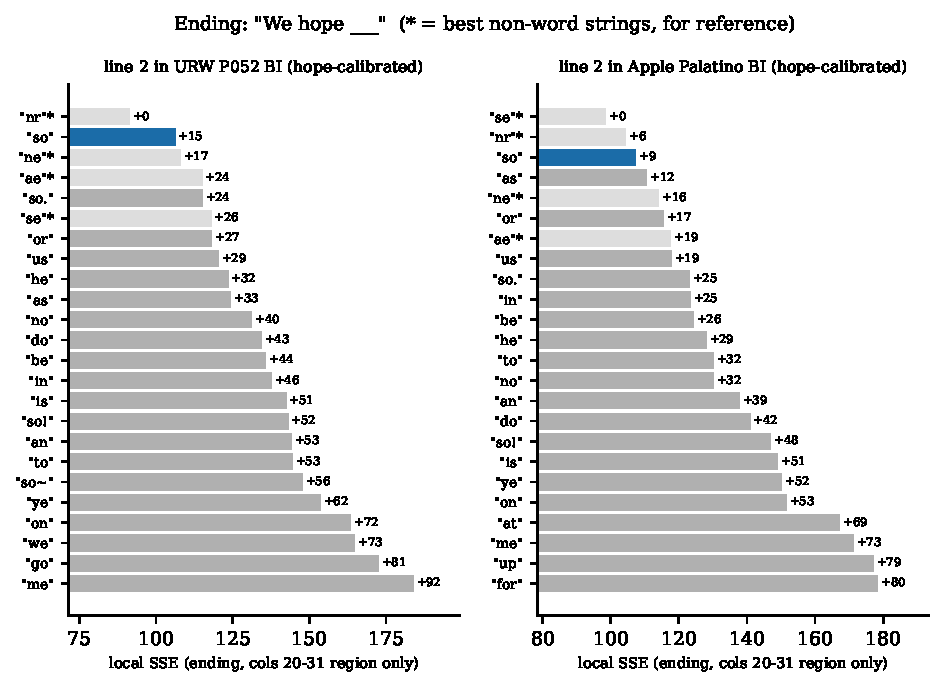
\includegraphics[width=0.95\linewidth]{hope_end_bars.pdf}
\caption{After calibrating line 2 on \q{hope}: local errors of first-word candidates (top) and ending candidates
(bottom).}
\label{fig:hopebars}
\end{figure}
\begin{figure}[p]\centering
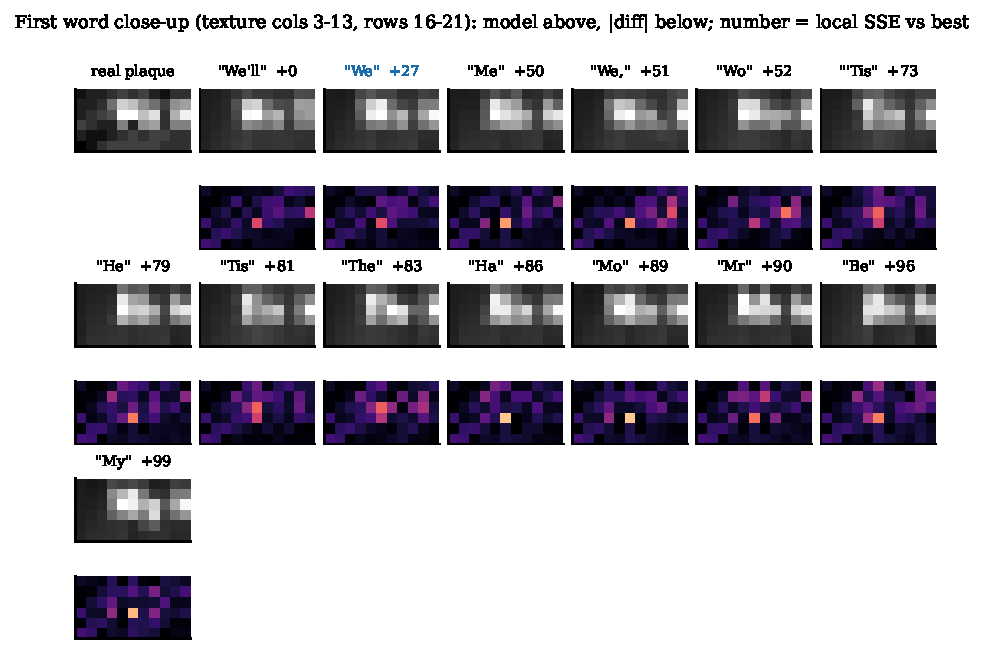
\includegraphics[width=\linewidth]{hope_first_crops.pdf}\\[2mm]
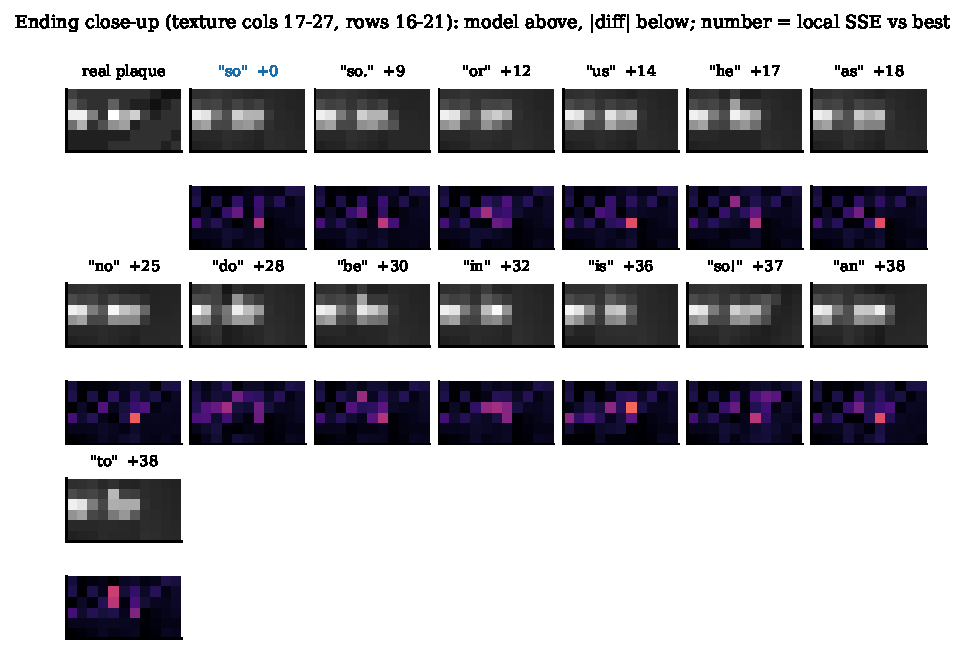
\includegraphics[width=\linewidth]{hope_end_crops.pdf}
\caption{Close-ups after the hope calibration (URW line 2): first word (top) and ending (bottom). Model above,
absolute difference below.}
\label{fig:hopecrops}
\end{figure}
\begin{figure}[p]\centering
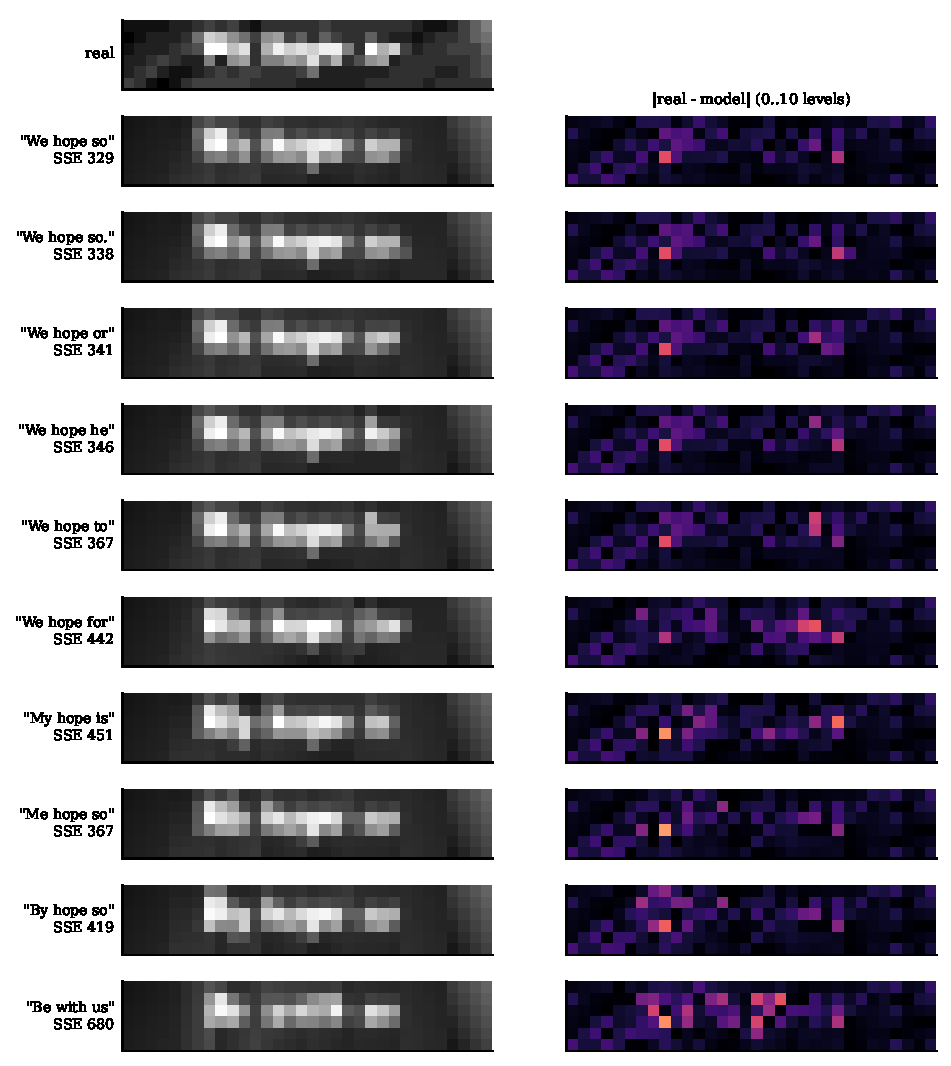
\includegraphics[width=0.9\linewidth]{hope_variant_panels.pdf}
\caption{Whole-line variants under the hope-calibrated line-2 typesetting (URW): real plaque (top), model (left) and
absolute difference (right).}
\label{fig:hopevariants}
\end{figure}
\begin{figure}[t]\centering
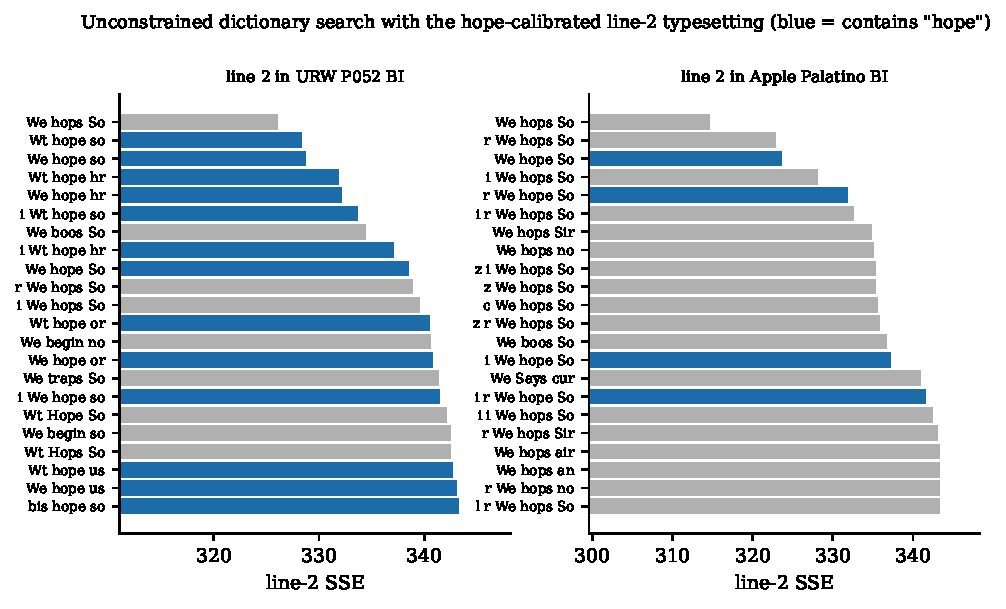
\includegraphics[width=0.98\linewidth]{hope_dp.pdf}
\caption{Unconstrained dictionary search under the hope-calibrated line-2 typesetting. \q{We \ldots so/So} now
emerges on its own.}
\label{fig:hopedp}
\end{figure}

%======================================================================================================
\section{Calibration: how much can the pixels tell?}
\label{sec:calib}
We planted \SimN{} known phrases into the real plaque. For each one we replaced the ink of the best reading by the
phrase's ink and kept the real stone and the real fit residual. We then decoded each plaque blind with the same
dictionary search (\cref{fig:sim}).
\begin{itemize}
\item \textbf{Exact recovery is rare.} The exact phrase came back first in \SimExact/\SimN{} cases, and
\SimWords{} words (\SimWordPct\,\%) were recovered. With a large vocabulary, some nonsense string often fits slightly
\emph{better} than the truth.
\item \textbf{The truth is never far from the optimum.} The true phrase always scored within $\approx$\,\SimMaxGap{}
\SSE{} of the best string found. This defines a \emph{pixel-compatible window}: readings more than about \SimMaxGap{} above the
optimum are effectively excluded, and readings inside it are distinguished by language.
\item \textbf{Strong words survive.} \q{hope} (or \q{hops}), \q{Shine}, \q{Thank you}, \q{happy} and \q{light} were
recovered well. Short function words and two-letter endings were not.
\end{itemize}

Under line~1's typesetting, the optimum for the real plaque is about 341--344.
\begin{itemize}
\item \textbf{Inside the window, in both fonts:} \q{We hope so} (373 Apple, 396 URW).
\item \textbf{Well outside:} \q{My hope is} (459--511), \q{No hope so} and \q{'Tis hope so} (466--474), and
\q{lie here\,\textasciitilde} (689--695).
\end{itemize}

\paragraph{Calibration under the hope-calibrated typesetting.}
We repeated the test with line~2's final typesetting from \cref{sec:hope} (\cref{fig:simhope}).
\begin{itemize}
\item \HSimExact/\HSimN{} phrases were recovered exactly and \HSimWordPct\,\% of words were recovered.
\item The truth always lay within \HSimMaxGap{} of the best string found.
\item On the real plaque, \q{We hope so} lies only \textbf{2.6} above the global optimum (328.7 vs.\ 326.1 for the
non-English \q{We hops So}). That is deep inside the window where, in simulation, the true text is found.
\end{itemize}

\begin{figure}[t]\centering
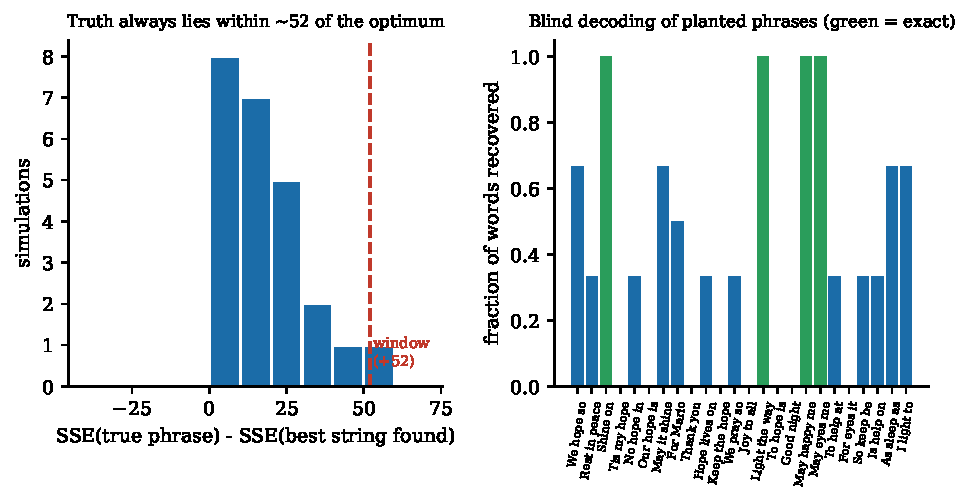
\includegraphics[width=0.95\linewidth]{simulation_hope.pdf}
\caption{Calibration under the hope-calibrated line-2 typesetting.}
\label{fig:simhope}
\end{figure}
\begin{figure}[t]\centering
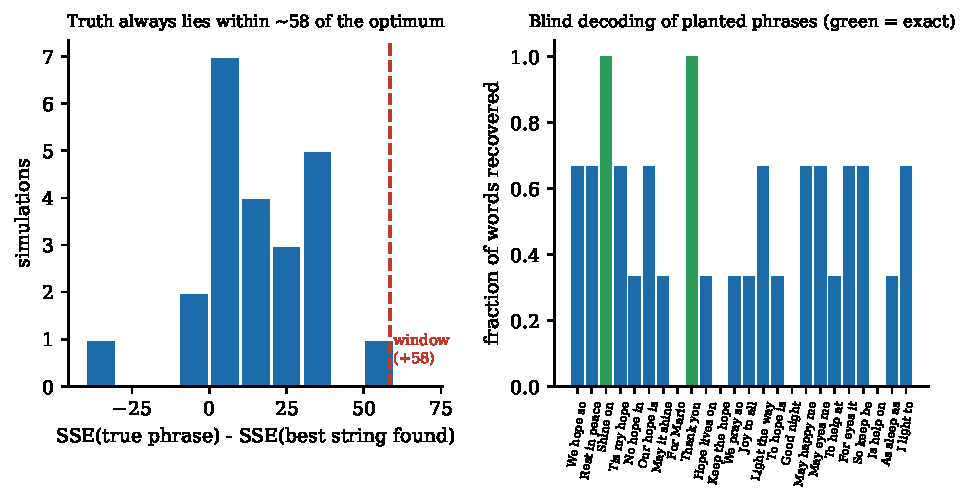
\includegraphics[width=0.95\linewidth]{simulation.pdf}
\caption{Calibration on synthetic plaques with known text: the gap between the true phrase and the best string found
(left), and the words recovered per simulation (right).}
\label{fig:sim}
\end{figure}



%======================================================================================================
\section{The artist's font file: Adobe's 1990 PostScript Palatino}
\label{sec:adobe}
The family is settled. We then asked which \emph{file} the artist used. Every digitisation of Palatino we could obtain
went through the identical pipeline: line-1 recipe search, then line~2 calibrated on \q{hope}
(\cref{tab:fontver,fig:fontver}).
\begin{itemize}
\item \textbf{URW Palladio}, the 1990s PostScript clone, in three generations: Ghostscript 5.10 (1998) and 6.0
(1999) from the GNU archive, and TeX Live's Palladio~L.
\item \textbf{TeX Gyre Pagella} and \textbf{URW P052}.
\item \textbf{Apple's System~7.5.3 Palatino} (1996).
\item \textbf{Palatino Linotype} (1998).
\item \textbf{Adobe's own Type~1 Palatino} (\texttt{Palatino-BoldItalic 001.005}, dated 2 July 1990), from an
\emph{Adobe Type Basics} disc of 1994. This copy was supplied by the reader and is not redistributed.
\end{itemize}

\paragraph{Adobe fits best.}
Adobe's original fits best on both lines: line~1 \AdobeLineOne{}, line~2 \AdobeLineTwo, total \AdobeTotal{} against
\AdobeNextTotal{} for the best clone, an improvement of \AdobeGain.
\begin{itemize}
\item \textbf{Recipe.} \AdobeCanvas{} canvas, \AdobeP\,px, tracking \AdobeTrack, blur \AdobeBlur, gamma
\AdobeGamma{}, at \AdobeRatio{} times the noise floor, the closest any rigid model came.
\item \textbf{Only Palatino benefits.} The other genuine Adobe fonts on the same disc (Times, New Century Schoolbook,
Garamond, Zapf Chancery, Bookman) do \emph{not} beat their clones. The Adobe advantage is specific to Palatino.
\item \textbf{Unhinted rendering is consistently worse.} The original was rasterised \emph{with} hinting, as Adobe Type
Manager did in 1996.
\end{itemize}

\paragraph{The blind search now finds the sentence by itself.}
With Adobe's Palatino, the unconstrained dictionary search over 17.7k English words returns exactly \textbf{\q{We hope
so}} as its single best string, in both settings (\cref{fig:adobedp}):
\begin{itemize}
\item line~1's typesetting: \AdobeDPTopSse, ahead of \q{\AdobeDPSecond};
\item hope-calibrated line~2: \AdobeDPHopeTopSse, ahead of \q{\AdobeDPHopeSecond}.
\end{itemize}
With every other font the top result had been a non-word such as \q{Wt hope he}. On its own pixels, \q{so} is now the
best of \emph{all} endings, non-words included (\AdobeEndSo{} vs.\ \q{nr} \AdobeEndNr). We conclude that the artist
most likely typeset the plaque with Adobe's PostScript Palatino Bold Italic, as found on Macintoshes with Adobe Type
Manager in the mid-1990s.

\paragraph{One pixel the fonts cannot explain.}
At the bottom of the \q{W} the real plaque shows bare stone (row~19, column~8; value~8) between two bright points
(\cref{fig:wzoom}). Every font predicts ink there, Adobe included (\AdobeHoleW). We tested and rejected global
explanations:
\begin{itemize}
\item full 1990s TrueType hinting;
\item sharpening after the resize;
\item a drop shadow or emboss;
\item 1996 Mac per-size advance widths;
\item unhinted rendering.
\end{itemize}
Moving only the W by one artwork pixel improves line~2 markedly (311 $\rightarrow$ 281 with Adobe) but does not empty the
hole. A second, similar hole sits between \q{Ete} and \q{rnal} on line~1. The most plausible explanation is the artist's
hand: manual kerning or a one-pixel touch-up of the finished 32$\times$32 texture, both common practice for tiny text.

\begin{table}[t]\centering\small
\IfFileExists{tables/fontver.tex}{\begin{tabular}{lrrrr}\toprule
 digitisation & line 1 & line 2 & total & hole (19,8) \\ \midrule
Palatino Bold Italic (Adobe Type 1, 1990) & 731.3 & 311.2 & 1042.5 & 14.8 \\
URW Palladio BI (Ghostscript 6.0, 1999) & 754.9 & 330.2 & 1085.1 & 14.1 \\
URW Palladio L BI (TeX Live) & 754.9 & 330.2 & 1085.1 & 14.1 \\
Palatino Bold Italic (URW P052) & 756.9 & 329.0 & 1085.9 & 14.2 \\
URW Palladio BI (Ghostscript 5.10, 1998) & 755.1 & 332.2 & 1087.4 & 14.1 \\
TeX Gyre Pagella BI & 756.6 & 331.5 & 1088.1 & 14.0 \\
Palatino Bold Italic (Apple 1996) & 759.2 & 350.4 & 1109.5 & 13.8 \\
Palatino Italic (Apple 1996) & 809.1 & 329.3 & 1138.4 & 14.3 \\
Palatino Linotype BI (1998) & 793.8 & 367.3 & 1161.1 & 15.2 \\
URW Palladio Italic (gs 5.10) & 804.3 & 391.6 & 1195.9 & 14.1 \\
Palatino Italic (Adobe Type 1) & 802.9 & 395.7 & 1198.5 & 14.1 \\
\bottomrule\end{tabular}
}{}
\caption{Palatino digitisations under the identical pipeline (hinted rendering). Lower is better. The last column is the
predicted value at the W hole; the real plaque shows 8.}
\label{tab:fontver}
\end{table}
\begin{figure}[t]\centering
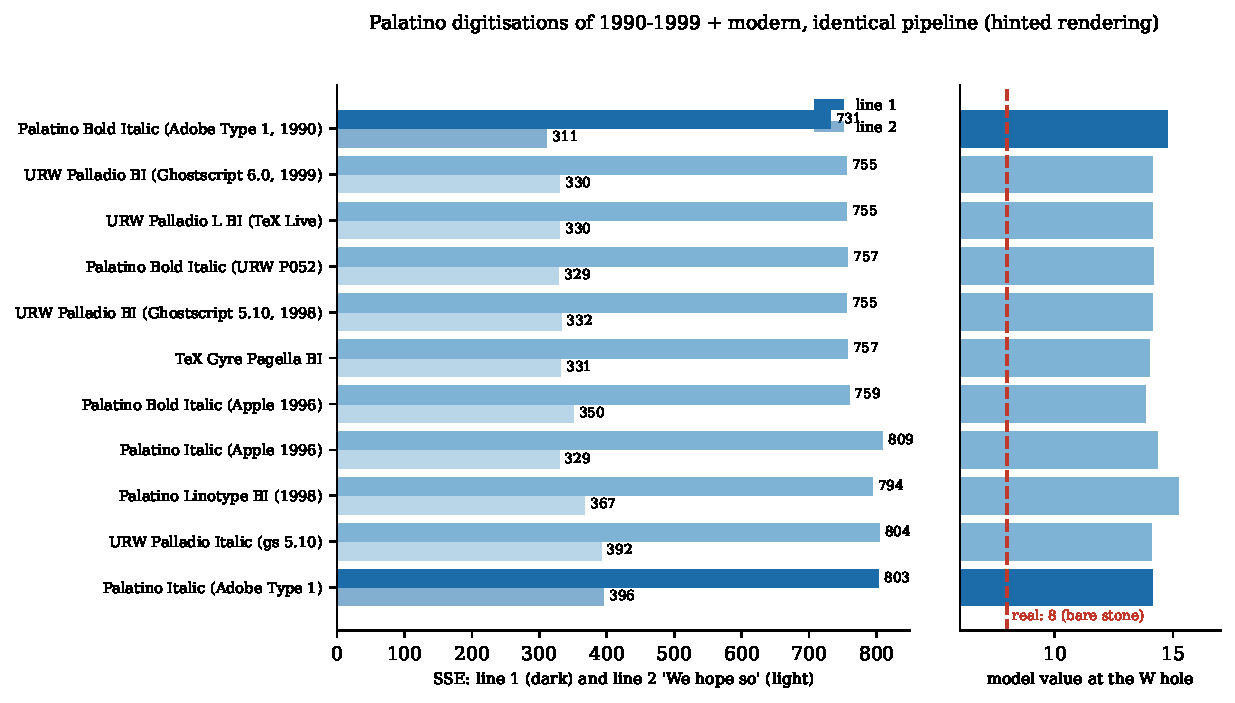
\includegraphics[width=\linewidth]{fontver.pdf}
\caption{Line-1 and line-2 errors for each Palatino digitisation (left) and the predicted value at the W hole (right).}
\label{fig:fontver}
\end{figure}
\begin{figure}[t]\centering
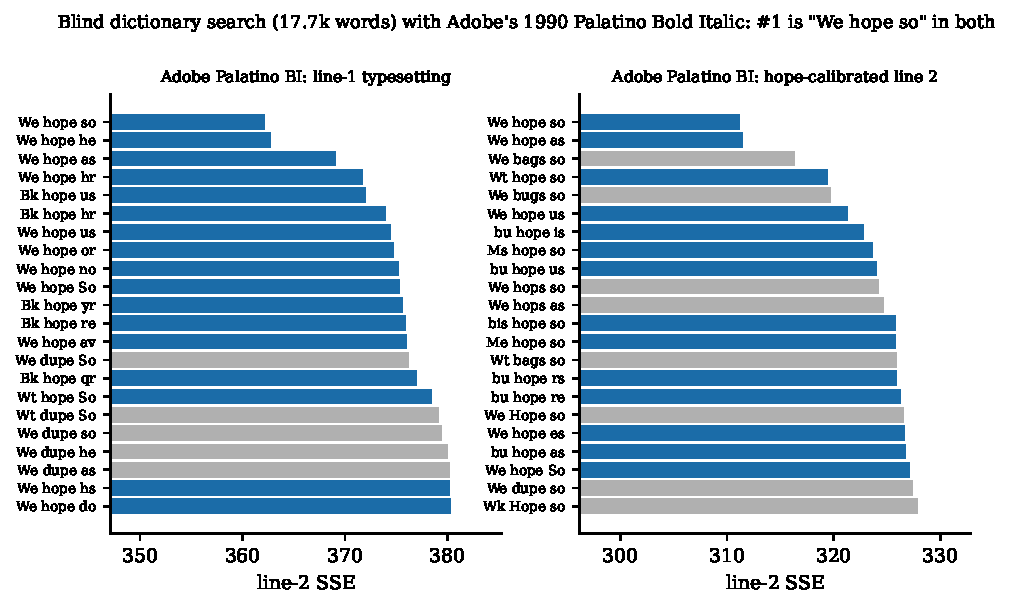
\includegraphics[width=0.98\linewidth]{adobe_dp.pdf}
\caption{Blind dictionary search with Adobe's 1990 Palatino Bold Italic. \q{We hope so} is the single best string of
the whole search, with line~1's typesetting (left) and with the hope-calibrated line~2 (right).}
\label{fig:adobedp}
\end{figure}
\begin{figure}[t]\centering
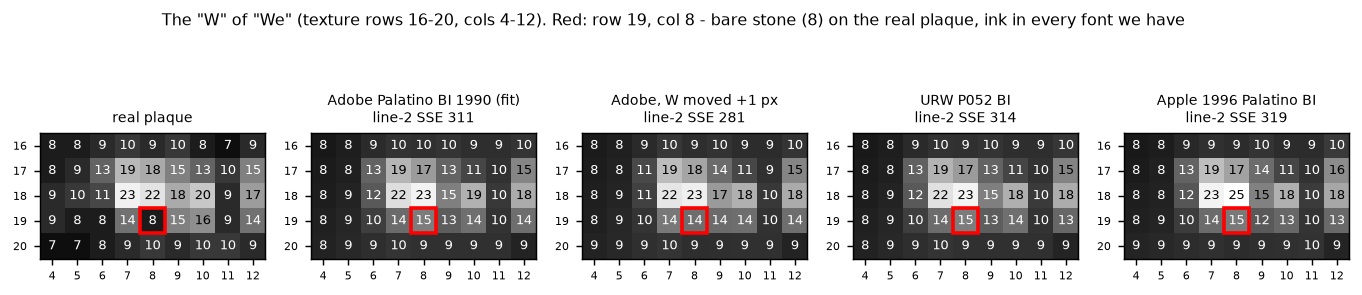
\includegraphics[width=\linewidth]{w_zoom.png}
\caption{The W of \q{We}, texture rows 16--20, columns 4--12, with grey levels printed. The red box marks the pixel
that is bare stone on the real plaque but inked in every font.}
\label{fig:wzoom}
\end{figure}

%======================================================================================================
\section{Inverting the process: can the text be made visible?}
\label{sec:invert}
The forward model maps a high-resolution artwork to the 32$\times$32 texture, so it can also be run backwards. We
solve for the 160$\times$128 artwork whose rendering, after the fitted resize, blur, gamma, ink level and stone removal,
reproduces the plaque.

\paragraph{Why priors are needed.}
\begin{itemize}
\item \textbf{Without a prior the problem is wildly underdetermined.} The inverse reproduces the texture
\emph{exactly} (residual 0), including its stone noise, and looks like noise (\cref{fig:invert}, column~2).
\item \textbf{Prior used.} We therefore add a sparsity and smoothness prior: most of the artwork is empty, and ink comes
in strokes. Optionally the ink is also pushed to be black or white.
\item \textbf{Setting its strength.} By the \emph{discrepancy principle}: the leftover error must equal the measured
noise floor of the two bands (331). The solver may then explain the ink, but not the noise.
\end{itemize}

\paragraph{Control plaques.}
A prior can draw letter-like strokes on its own, so we apply the \emph{identical} inversion to synthetic plaques with
known text.
\begin{itemize}
\item \textbf{Construction.} Every hypothesis gets the same smooth stone and the same real stone noise, taken from the
clean rows 23--31. For \q{L is real 2401}, row~2 keeps the real pixels because that claim says nothing about it.
\item \textbf{Text is recoverable in principle.} On these plaques the inversion returns legible text (\q{Eternal Star},
\q{L is real 2401}, \q{A Secret star}). A correctly modelled plaque at this noise level could therefore be partly
\q{read} after inversion.
\item \textbf{The real plaque is less legible.} It inverts to letter-like blobs with the word structure \q{E ternal
star / We hope so}. The cause is not noise but the remaining model mismatch of \cref{sec:process}: the real 1996 letter
spacing and rasterising differ slightly from our fonts.
\end{itemize}

\paragraph{Similarity to the hypotheses.}
The correlation between the real inversion and each synthetic inversion, in the artwork space, is:
\begin{itemize}
\item row~1: \textbf{\InvOursOne} for \q{Eternal Star} vs.\ \InvLisRealOne{} for \q{L is real 2401} and \InvSecretOne{}
for \q{A Secret star};
\item row~2: \textbf{\InvOursTwo} for \q{We hope so} vs.\ \InvMyHopeTwo{} for \q{My hope is} and \InvSecretTwo{} for
\q{lie here\,\textasciitilde}.
\end{itemize}
The inverted plaque looks like the inversion of \q{Eternal Star / We hope so} and clearly unlike the published
alternatives. This is consistent with, and independent of, the forward scoring in the previous sections.

\begin{figure}[t]\centering
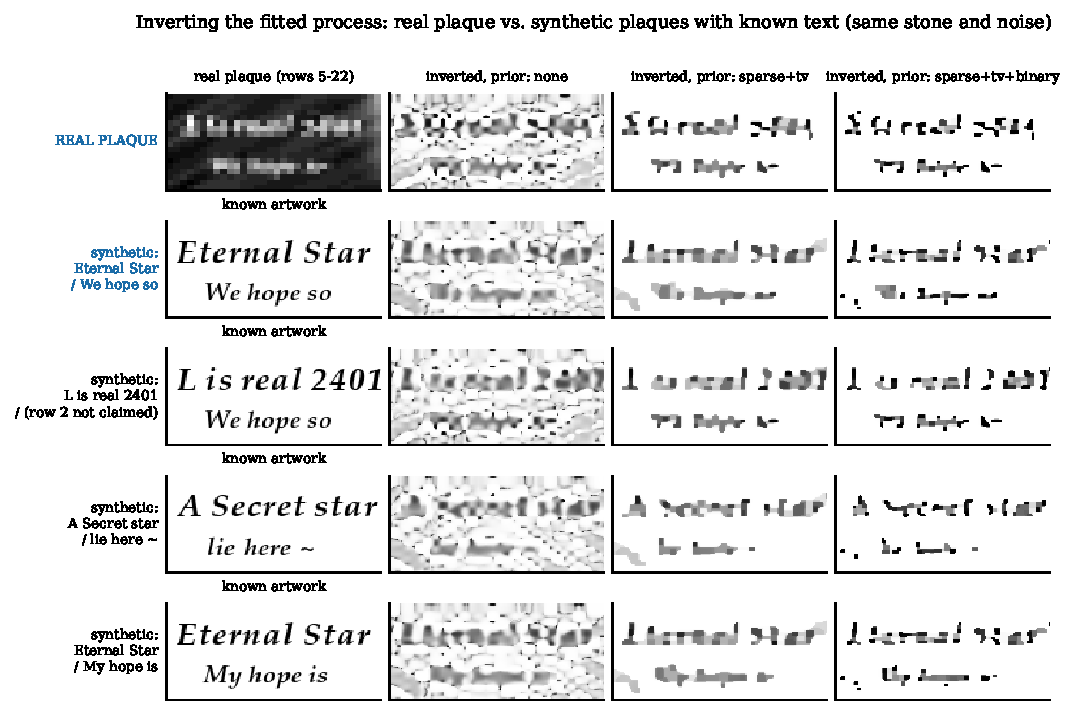
\includegraphics[width=\linewidth]{inversion.pdf}
\caption{Inverting the fitted process. Top row: the real plaque and its inversion with three priors. Other rows:
synthetic plaques with known artwork (left) on the same stone and noise, inverted identically. Column~2 (no prior)
reproduces the pixels exactly but is meaningless. Columns 3--4 use the prior strength that leaves exactly the noise
floor.}
\label{fig:invert}
\end{figure}

%======================================================================================================
\section{Second pass: the plain stone, every string and every era font}
\label{sec:stone}
Readers asked three things: can the stone be taken out of the fit, does a non-word or a word outside our lists fit
better, and was Palatino really the font available to the artist? We answered each directly.

\paragraph{The plain stone.}
Every pixel outside two boxes drawn around the visible text is stone and is kept unchanged (line~1: rows 8--12,
columns 2--29; line~2: rows 16--20, columns 6--24; 235 of 1{,}024 pixels). Inside the boxes the stone is filled by
Gaussian-process inpainting from all other pixels: an anisotropic kernel along the visible streaks (bottom left to top
right; 10\,px along, 4.5\,px across) plus a quadratic trend (\cref{fig:stonebox}; \texttt{python -m plaquedecode
stone}). The model is then scored as $\sum_i w_i\,(t_i - s_i - L\,c_i)^2$ with the stone $s$ fixed and
$w_i = 1/(0.15 + \operatorname{var}(s_i))$, so the stone can no longer absorb ink.

\begin{figure}[t]\centering
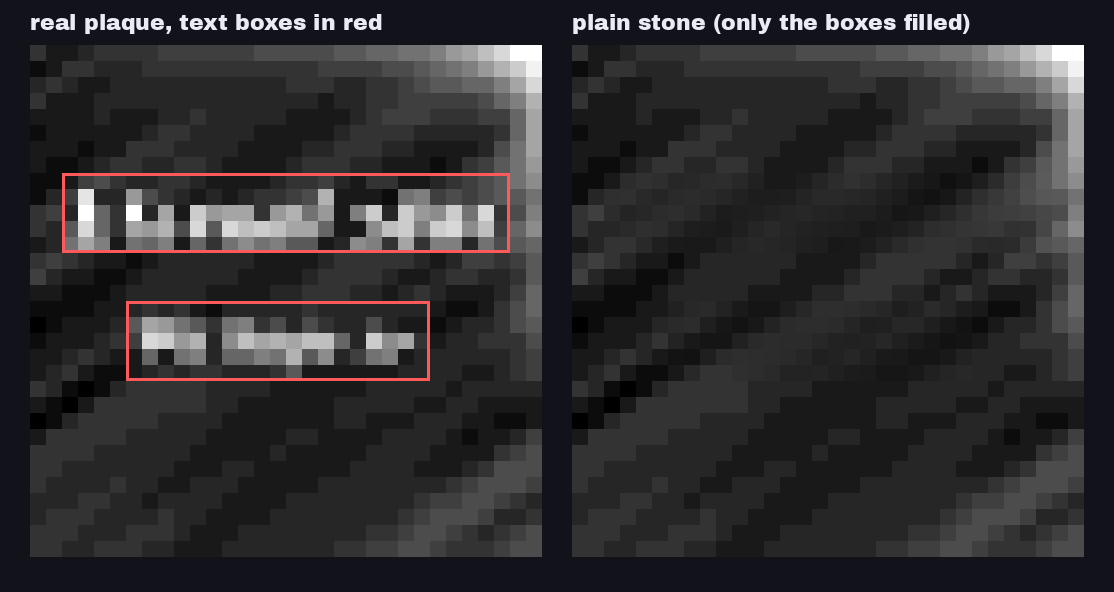
\includegraphics[width=0.78\linewidth]{stone_box.png}
\caption{The text boxes (left) and the plain stone (right): only the 235 pixels inside the boxes are filled; every
other pixel is the plaque itself.}
\label{fig:stonebox}
\end{figure}

\paragraph{Same recipe, same words.}
\begin{itemize}
\item The recipe search against the fixed stone returns exactly the Adobe recipe of \cref{sec:adobe} (26\,px,
192$\times$160, tracking +2, bilinear, blur 0.3, gamma 1.4; \SSE~\StoneStar). Apple's and URW's best recipes are
unchanged as well (\cref{tab:recipe}).
\item Word~2: \q{Star} is the best of \SwTwoN{} words (\SwTwoTop). Among \SwBigN{} entries of a large multilingual
list it ranks \SwBigRank{} (\SwBigTop): only the Italian \q{stai} and the Scandinavian \q{stor} come before it.
\item Rival texts in the same font and process: \q{Eternal star} \StoneLower, \q{L is real 2401} \StoneLegend,
\q{A Secret star} \StoneSecret.
\end{itemize}

\paragraph{Every string, not just words.}
We scored \q{Eternal~} followed by \emph{every} string of three or four letters (first letter in either case; \ExN{}
strings, four word spaces each) exactly, with linear glyph tiles under the frozen recipe. \q{Star} ranks
\ExRankStar{}; all strings ahead of it share its shape, \q{St/Sl} + a round letter + a short letter (\ExTop). The
third and fourth letters (a/o, r/i) are not separable at this resolution; the pixels force \q{St} + round + short
letter, and \q{Star} is the only common word of that shape. On line~2 every slot was opened the same way:
\begin{itemize}
\item first word, all \ExFirstN{} strings of 1--3 letters: \q{We} ranks \ExFirstRank{} behind W-shaped non-words
(\ExFirstTop);
\item ending, all \ExEndN{} strings: \q{so} ranks \ExEndRank{} (\ExEndTop);
\item middle word, all \ExMidN{} four-letter strings: \q{hope} ranks \ExMidRank{} (\ExMidTop).
\end{itemize}
Each slot lands in the top 0.01\,\% of all strings, and in each case the strings ahead are the same shape class
(b and h are not separable at 3.5\,px). The pixels fix the shapes; the language picks the words.

\paragraph{Was Palatino available to the artist?}
We read every package of the IRIX~5.3 installation CD for the Indy (August 1995; SGI workstations were the N64
development platform). IRIX ships Adobe Times, Helvetica, Courier, Symbol and Utopia, Bitstream Charter and 14 SGI
display faces, but no Palatino. Two details link Palatino to it anyway:
\begin{itemize}
\item SGI's online-documentation viewer expects \texttt{/usr/lib/DPS/outline/base/Palatino-BoldItalic} (symbolic links
in \texttt{insight.sw}), together with New Century Schoolbook and Zapf Chancery.
\item IRIX's printing package installs \texttt{/usr/sbin/typeoncall}, \q{TypeOnCall for IBM PC CD-ROM}: it unlocks
fonts from Adobe's PC \emph{Type On Call} disc and converts their \texttt{.PFB} files into that directory.
\end{itemize}
That disc's \texttt{POBI\_\_\_\_} metrics file is byte-identical to the one that accompanies the Adobe 1990 file used
here. The Palatino Bold Italic an SGI artist could install in 1995 was therefore exactly this Adobe 001.005 face.

\paragraph{\EraN{} era faces under one process.}
We then collected every outline face an artist could plausibly have had in 1993--1996 from operating systems and
bundled applications: IRIX~5.3 (including Showcase), Adobe Illustrator~5.5 for IRIX (221 Adobe/ITC faces),
the 1990 Adobe Type~1 disc, CorelDRAW~6/7 (the Bitstream library), Microsoft Office~4.3, Font Pack~2 and Bitstream
TrueType packs, Apple KanjiTalk~7.5, System~7.5.3 and Mac OS~9, Photoshop~3 (ATM), FreeHand~5, and Windows~3.1/95
(Japanese). All \EraN{} italic faces ran through the same recipe search in three tiers (a quick grid for all, the
font-comparison grid for the top 60, the full grid for the top 8). The best is Adobe's 1990 Palatino Bold Italic
(\EraBest); the twelve best distinct faces are all Palatino digitisations or close Palatino derivatives (\cref{tab:erafonts,fig:erafonts}).
The best face of any other design is \EraOther{} at \EraOtherSse; IRIX's own Times Bold Italic is at 1{,}116.

\begin{table}[t]\centering\small
\IfFileExists{tables/era_fonts_stone.tex}{\begin{tabular}{rllrl}\toprule
\# & face & source & SSE & recipe \\ \midrule
1 & Palatino Bold Italic 001.005 & Adobe Type 1, 1990 & 788.7 & 26 px, 192$\times$160, $\gamma$ 1.4 \\
2 & Palatino Bold Italic 003.001 & Adobe Type 1, 1999 & 808.3 & 32 px, 192$\times$192, $\gamma$ 1.4 \\
3 & Palatino Bold Italic & Apple System 7.5.3 / KanjiTalk 7.5 & 811.4 & 23 px, 160$\times$128, $\gamma$ 1.8 \\
4 & Palatino Bold Italic 3.5a3 & Apple Mac OS 9 & 811.4 & 23 px, 160$\times$128, $\gamma$ 1.8 \\
5 & P052 Bold Italic & URW clone & 814.0 & 32 px, 192$\times$192, $\gamma$ 1.4 \\
6 & Palladio L Bold Italic & URW clone (TeX Live) & 821.4 & 23 px, 160$\times$128, $\gamma$ 1.8 \\
7 & URW Palladio Bold Italic & URW clone (Ghostscript 6.0) & 821.4 & 23 px, 160$\times$128, $\gamma$ 1.8 \\
8 & URW Palladio Bold Italic & URW clone (Ghostscript 5.10) & 822.2 & 23 px, 160$\times$128, $\gamma$ 1.8 \\
9 & Zapf Calligraphic 801 Bold Italic & Bitstream & 847.1 & 26 px, 192$\times$160, $\gamma$ 1.4 \\
10 & Palatino Linotype Bold Italic & Linotype, 1998 & 859.3 & 32 px, 192$\times$192, $\gamma$ 1.4 \\
11 & Book Antiqua Bold Italic & MS TrueType Font Pack, 1992 & 884.5 & 27 px, 192$\times$160, $\gamma$ 1.4 \\
12 & Zapf Calligr BT Italic & CorelDRAW 6 (Bitstream) & 896.4 & 31 px, 192$\times$192, $\gamma$ 1.8 \\
13 & Schneidler Blk BT Black Italic & CorelDRAW 6 (Bitstream) & 926.4 & 36 px, 256$\times$192, $\gamma$ 1.8 \\
14 & Dutch 811 BT Bold Italic & CorelDRAW 6 (Bitstream) & 946.1 & 25 px, 192$\times$160, $\gamma$ 1.4 \\
15 & Lapidary 333 BT Bold Italic & CorelDRAW 6 (Bitstream) & 950.6 & 32 px, 192$\times$160, $\gamma$ 1.4 \\
16 & Book Antiqua Italic & MS Office 4.3 & 953.6 & 27 px, 192$\times$160, $\gamma$ 1.4 \\
17 & Century Expd BT Bold Italic & CorelDRAW 6 (Bitstream) & 954.3 & 31 px, 256$\times$192, $\gamma$ 1.4 \\
18 & Bodoni Bold BT Bold Italic & CorelDRAW 6 (Bitstream) & 961.2 & 35 px, 256$\times$192, $\gamma$ 1.0 \\
19 & Palatino Italic 001.005 & Adobe Type 1, 1990 & 973.2 & 27 px, 192$\times$160, $\gamma$ 1.4 \\
20 & C059 Bold Italic (New Century Schoolbook) & URW clone & 980.7 & 21 px, 160$\times$128, $\gamma$ 1.8 \\
\bottomrule\end{tabular}
}{}
\caption{Line~1 against the plain stone, best recipe per face (\EraN{} faces; identical files merged).}
\label{tab:erafonts}
\end{table}
\begin{figure}[t]\centering
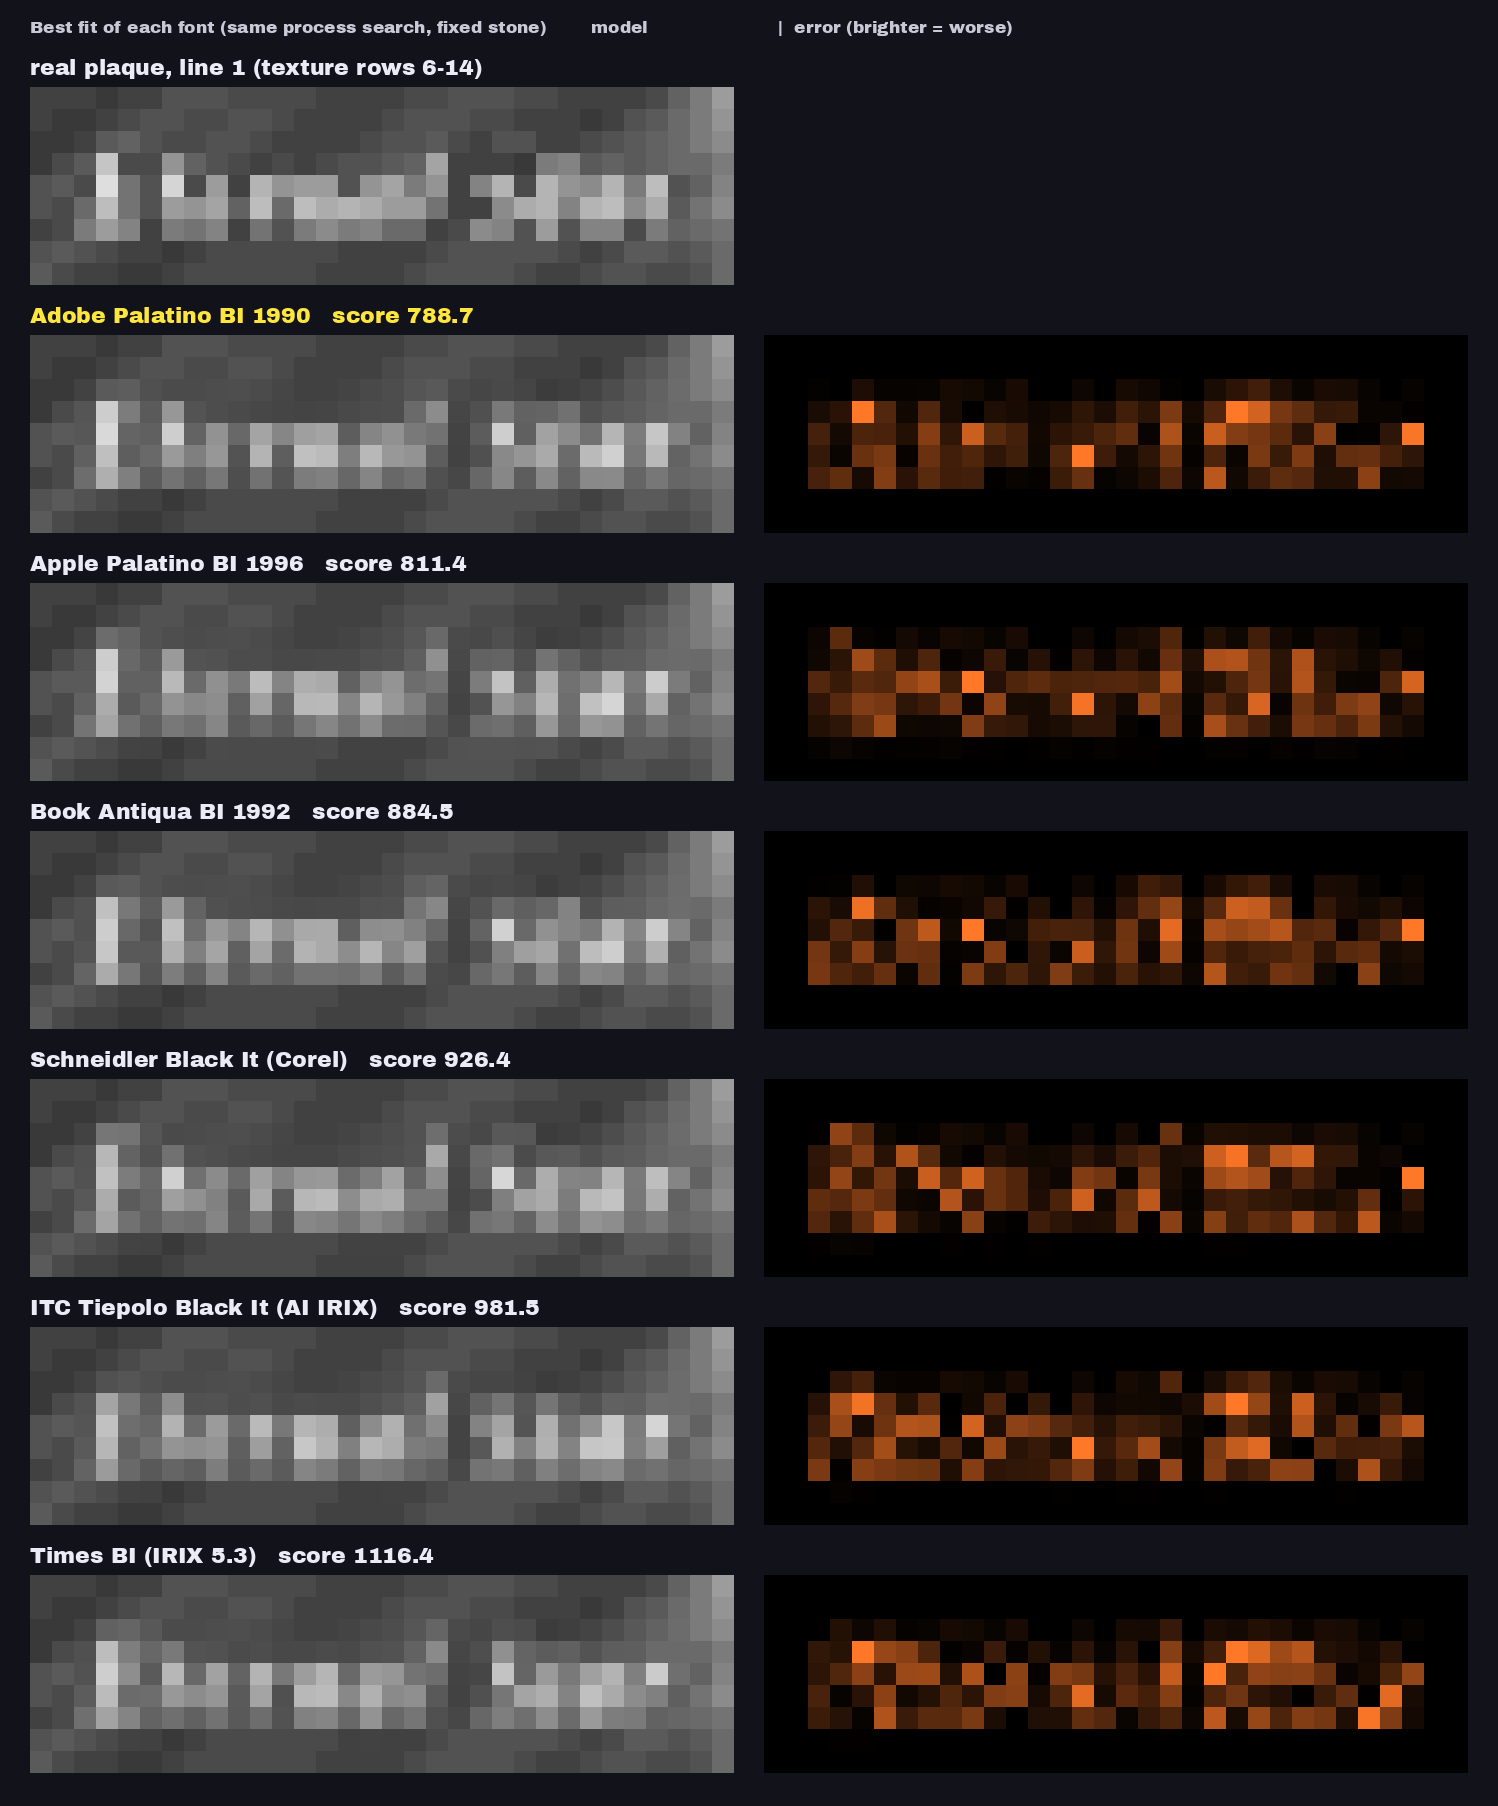
\includegraphics[width=0.85\linewidth]{era_font_compare.png}
\caption{Line~1: the real plaque, each font's best fit and its error map (brighter = worse).}
\label{fig:erafonts}
\end{figure}

\paragraph{What is left.}
With the stone fixed, the remaining large errors sit on the \emph{top} strokes of line~1 (E top arm, S top, the r
arm) and in the W of line~2, where the model inks pixels the plaque shows as bare stone. To explain them by the stone
it would have to be darker than any stone pixel on the plaque; per-letter vertical shifts do not beat a noise-only
control. Horizontal per-letter shifts do; \cref{sec:designer} follows this up like a designer would.

%======================================================================================================
\section{Third pass: thinking like the designer}
\label{sec:designer}
So far every letter sat exactly where the font put it. A real artist in 1996 typed the text, looked at it, nudged
letters, maybe added an effect, and only then shrank the artwork to 32$\times$32. We now let the model do the same
things and ask, for every step, one question: \emph{does it help more on the real plaque than on pure noise?}

\paragraph{How we decide that a step is real.}
Any extra freedom lowers the error a little, even on random data. So for every step we also build \emph{fake
plaques}: our best model plus the real plaque's leftover error, shuffled to random positions. A fake looks like the
plaque but contains no hidden structure. We run exactly the same search on several fakes. A step counts as real only
if it helps the real plaque clearly more than it helps every fake.

\paragraph{Step 1: hand kerning.}
Each letter may move left or right by whole pixels of the artwork, the way an artist nudges letters with the arrow
keys (one artwork pixel is a sixth of a texture pixel). Line~1 improves from \NgOneRigid{} to \NgOneKern{} (fakes:
\NgOneNoise), line~2 from \NgTwoRigid{} to \NgTwoKern{} (fakes: \NgTwoNoise). Both gains are far above the fakes:
the letters really were placed slightly differently than the font places them. In line~2 the nudges pull \q{so}
slightly to the left and move the W slightly right. We also searched every one of the 2{,}000 best recipes with
hand kerning allowed: the winner is the same recipe (26\,px, 192$\times$160, tracking +2, bilinear), so kerning does
not change the font, the size or the process, only the letter positions.

\paragraph{Step 2: one canvas for both lines.}
Both lines are now typed on the same artwork, kerned together and shrunk together, with one ink level per line:
\DzPlain{} before kerning, \DzKern{} after.

\paragraph{Step 3: everything else a designer could have done.}
\Cref{tab:designer,fig:designersteps} list each step with its gain on the real plaque and on the fakes.
\begin{table}[t]\centering\small
\begin{tabular}{p{5.4cm}rrl}\toprule
designer step & gain (real) & gain (fakes) & verdict\\\midrule
text layer blended with the stone as \q{Screen} (or \q{Normal}) & \DzBlendGain & \DzBlendNoise & not real\\
text layer blended as \q{Lighten} & \multicolumn{2}{l}{much worse (\DzLighten)} & ruled out\\
engraved / drop shadow & \DzShadowGain & \DzShadowNoise & not real\\
emboss / bevel & \DzEmbossGain & \DzEmbossNoise & borderline\\
outline around the letters & \DzOutlineGain & \DzOutlineNoise & no\\
sharpen after shrinking & \DzSharpenGain & \DzSharpenNoise & no (worse)\\
move a whole line up or down & \DzLineGain & \DzLineNoise & no (worse)\\
artwork \DzScaleW$\times$\DzScaleH{} instead of 192$\times$160, re-kerned & \DzScaleGain & \DzScaleNoise & \textbf{real}\\
\bottomrule\end{tabular}
\caption{Designer steps on top of the hand-kerned two-line canvas. \q{Gain} is how much the error drops.}
\label{tab:designer}
\end{table}
\begin{figure}[t]\centering
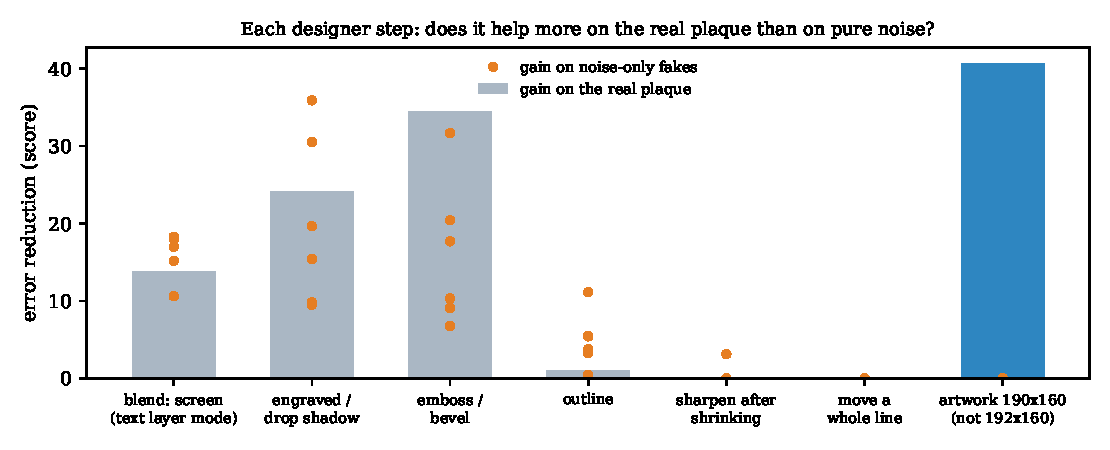
\includegraphics[width=0.95\linewidth]{designer_steps.pdf}
\caption{Blue bars: gain on the real plaque; orange dots: gain on noise-only fakes. Only the slightly narrower
artwork (and the hand kerning before it) clearly beats noise.}
\label{fig:designersteps}
\end{figure}
The one step that clearly survives is the artwork size. Our recipes assumed artwork exactly 6$\times$5 times the
texture (192$\times$160). Allowing any artwork size between 176 and 208 pixels wide and 136 and 184 high, the best is
\textbf{\DzScaleW$\times$\DzScaleH}: about 1\,\% narrower, error \DzScaleInt{} $\to$ \DzScaleBest; on the fakes this
freedom bought nothing. The text was set a little tighter than the font sets it, which the hand kerning had already
hinted at.

\paragraph{The best version.}
Our best reconstruction is therefore: Adobe Palatino Bold Italic (1990), line~1 at 26\,px and line~2 at 19\,px, typed
on one 190$\times$160 artwork, letters nudged by at most a third of a texture pixel, shrunk to 32$\times$32 with a
bilinear filter, light blur and gamma 1.4, on the extracted stone (\cref{fig:designerlines}; the README's title image).
Inside the two text boxes the model is on average 1.1 grey levels away from the plaque (out of 31); 83\,\% of the
text pixels are within 2 levels.

\begin{figure}[t]\centering
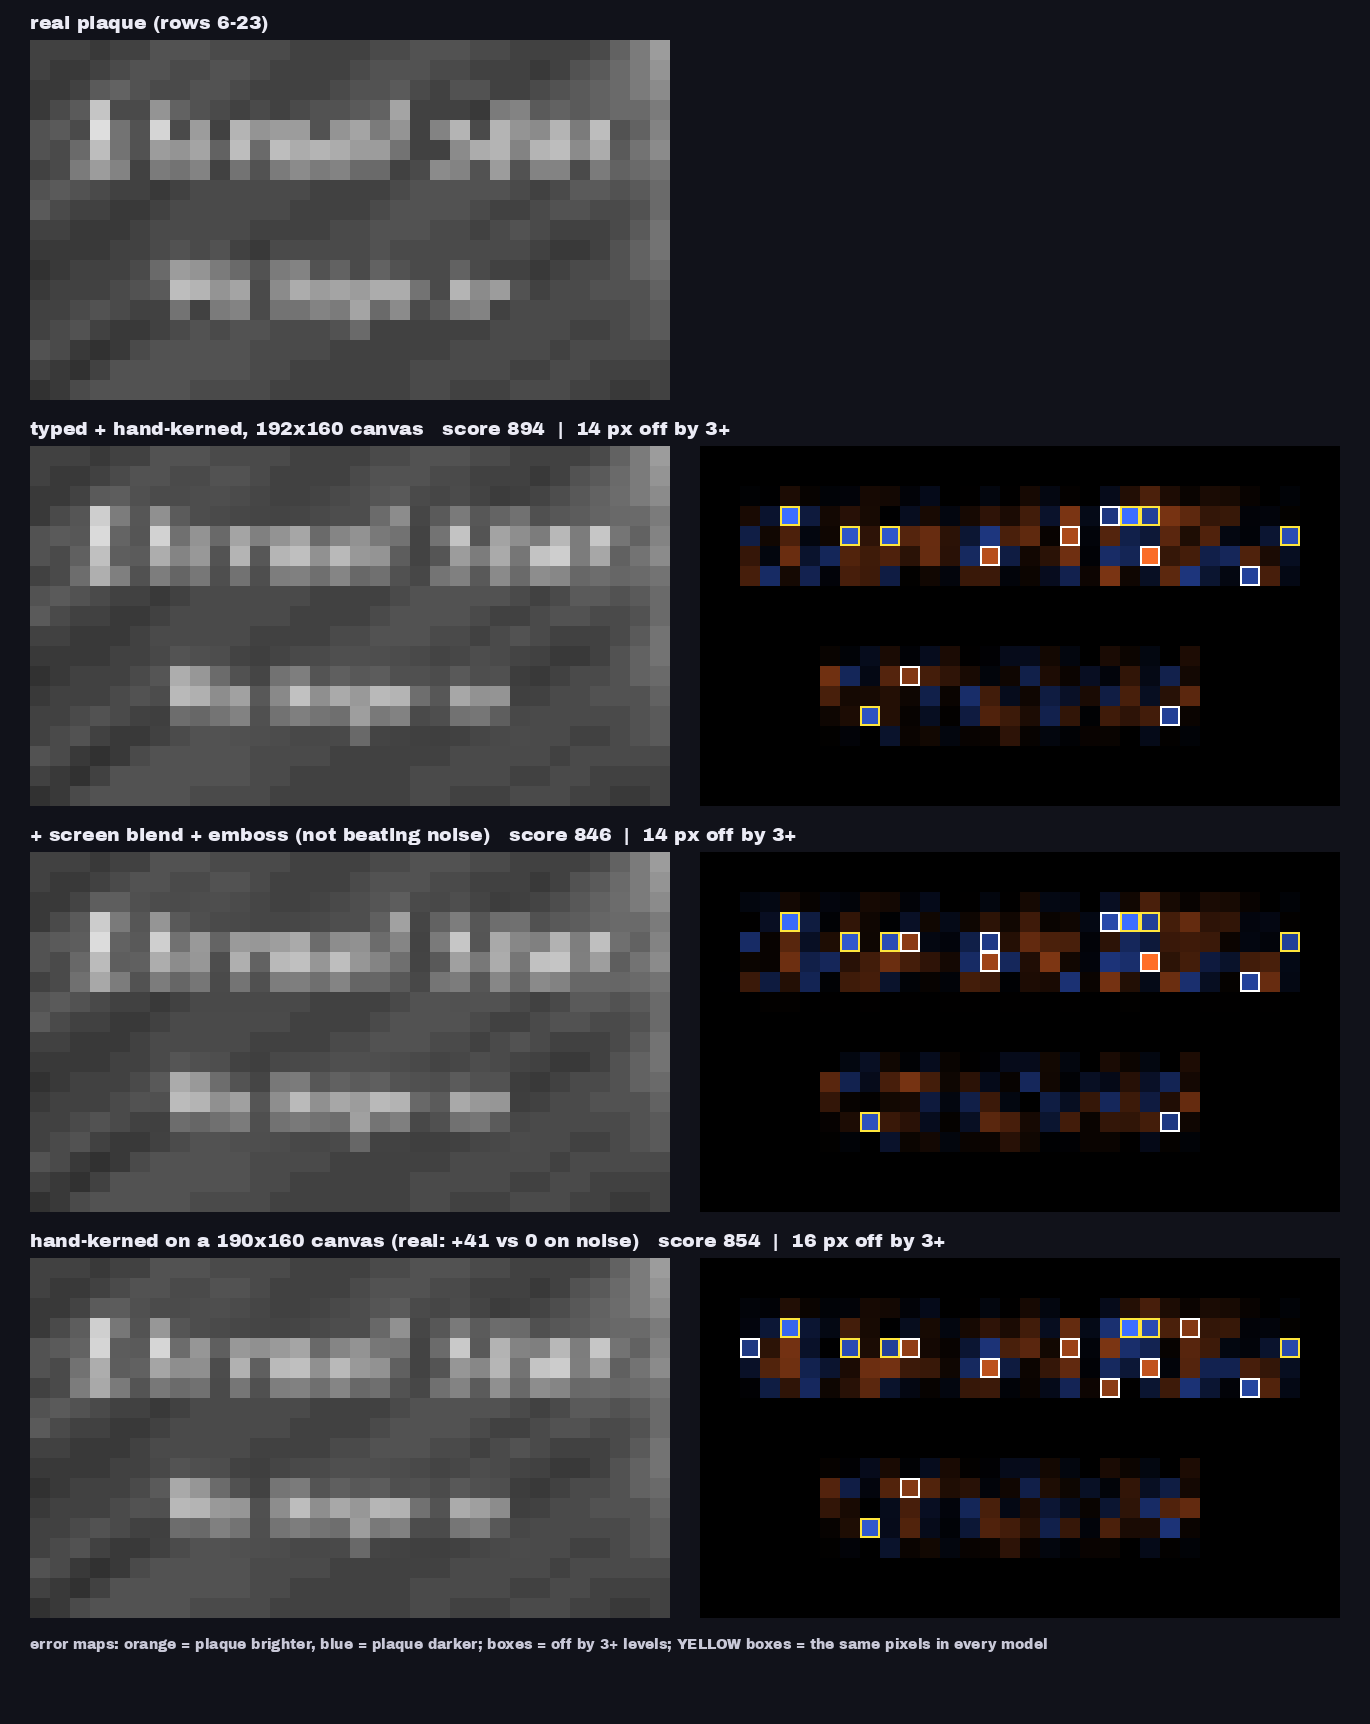
\includegraphics[width=0.95\linewidth]{designer_both_lines.png}
\caption{Both lines: the real plaque, the hand-kerned model, the model with the (not significant) blend and emboss
steps, and the hand-kerned model on the 190$\times$160 artwork. Right: error maps. Yellow boxes mark the pixels that
stay wrong in every model.}
\label{fig:designerlines}
\end{figure}

\paragraph{What no designer step explains.}
The same seven pixels stay wrong in every version (yellow in \cref{fig:designerlines}): the top arm of the E, two
pixels on top of the S, two pixels around the first \q{t}, the arm of the r, and the gap at the bottom of the W. At
each of them the plaque shows bare stone while every typeset version predicts faint grey ink. No font, size,
filter, blend mode or effect removes exactly these pixels without breaking others. The simplest explanation is that
the artist touched up the finished 32$\times$32 texture by hand and cleaned away a few faint grey edge pixels. This
cannot be modelled from the font, and it changes nothing about the reading.

%======================================================================================================
\section{Comparison with published readings}
\label{sec:claims}
Every claim was scored with the same model. Each claimed line~1 received its \emph{own} exhaustive recipe search. Line~2
was scored jointly under that recipe, and also under the \q{Eternal Star} recipe. The results are in \cref{tab:claims},
\cref{fig:claims} and \cref{fig:claimpanels}.

\begin{table}[t]\centering\footnotesize
\IfFileExists{tables/claims.tex}{\begin{tabular}{>{\raggedright\arraybackslash}p{2.7cm}>{\raggedright\arraybackslash}p{2.0cm}>{\raggedright\arraybackslash}p{4.0cm}rrrr}\toprule
 line 1 & line 2 & proposed by & \multicolumn{2}{c}{line-1 SSE} & \multicolumn{2}{c}{line-2 SSE} \\
 & & & Apple & URW & Apple & URW \\ \midrule
``L is real 2401'' & (not claimed) & 1990s rumour ('Luigi is real'), whole phrase on row 1 & 1492 & 1414 & -- & -- \\
``L is real 2041'' & (not claimed) & variant spelling, row 1 (e.g. MobyGames trivia) & 1561 & 1437 & -- & -- \\
``A Secret star'' & ``lie here \textasciitilde{}'' & Daniel Nodd (No64DD), Nintendo Life & 1604 & 1460 & 1126 & 1320 \\
``L is real star'' & (not claimed) & reader comment, Nintendo Life & 1421 & 1378 & -- & -- \\
``Eternal Star'' & (not claimed) & Super Mario Wiki ('more likely') & 759 & 757 & -- & -- \\
``Eternal Star'' & ``My hope is'' & proposed reading (two descenders + ascender) & 759 & 757 & 511 & 459 \\
``Eternal Star'' & ``my hope is'' & same, lower case & 759 & 757 & 489 & 475 \\
``Eternal Star'' & ``lie here \textasciitilde{}'' & Nodd's line 2 under Eternal Star & 759 & 757 & 695 & 689 \\
``Eternal Star'' & ``We hope so'' & this work & 759 & 757 & 373 & 396 \\
``Eternal star'' & ``We hope so'' & this work (lower-case s) & 765 & 755 & 554 & 565 \\
\bottomrule\end{tabular}
}{(generated by \texttt{plaquedecode claims})}
\caption{Published and proposed readings. Lower is better. Line-1 noise floor 165.7. The line-2 pixel-compatible window
is roughly \WindowLo--\WindowHi.}
\label{tab:claims}
\end{table}
\begin{figure}[t]\centering
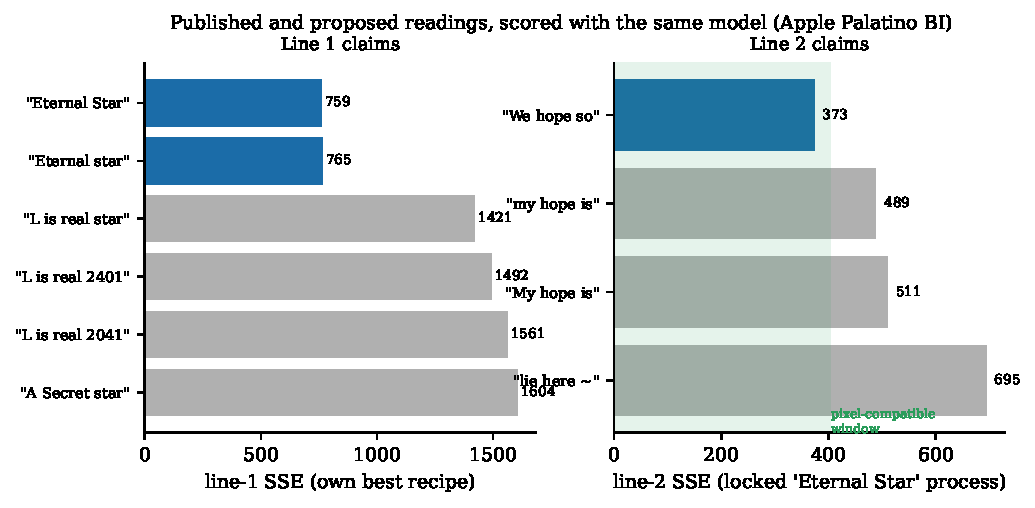
\includegraphics[width=\linewidth]{claims.pdf}
\caption{Line-1 and line-2 errors of the claims. The green band is the line-2 pixel-compatible window.}
\label{fig:claims}
\end{figure}
\begin{figure}[p]\centering
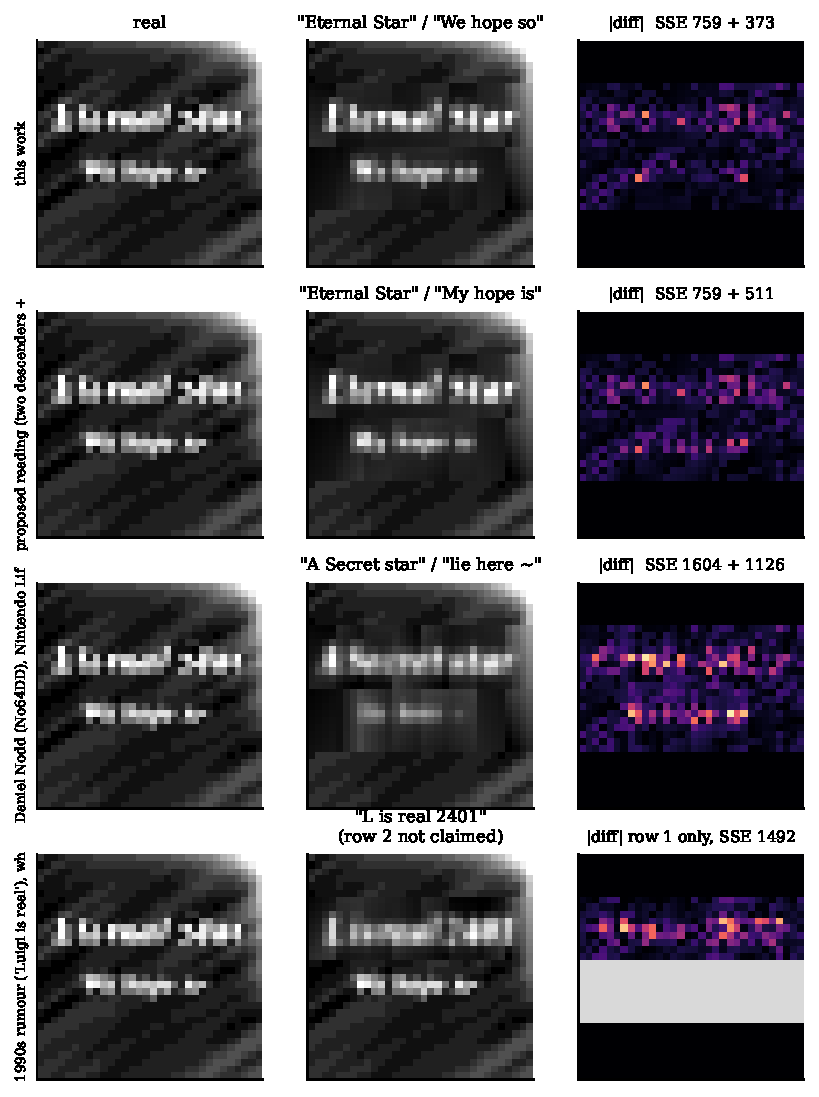
\includegraphics[width=0.86\linewidth]{claim_panels.pdf}
\caption{Whole-plaque reconstructions of four readings: real plaque, model rendering and absolute difference.}
\label{fig:claimpanels}
\end{figure}

\paragraph{\q{L is real 2401}.}
The legend puts the whole phrase on row~1 and makes no claim about row~2, so we scored it that way. Row~1 received its
own exhaustive recipe search, and row~2 was not scored.
\begin{itemize}
\item \textbf{Row~1 fit.} Even so, \q{L is real 2401} fits row~1 about twice as badly as \q{Eternal Star}: \ClaimLisRealOne{}
(Apple) against 759. The \q{2041} spelling does the same (\ClaimLisRealAltOne).
\item \textbf{Why.} The texture shows a long, evenly inked first word with a tall capital at the start and no gap after
it. \q{L is} predicts a short capital L and a two-letter word separated by spaces, and the digits predict wide,
cap-height shapes where the texture has italic lower-case letters (\cref{fig:claimpanels}).
\item \textbf{Row~2.} Its text is left unexplained by this reading.
\end{itemize}
Our results agree with the 1998 Nintendo letter that the legend has no basis in the texture~\cite{mnn}.

\paragraph{\q{A Secret star / lie here\,\textasciitilde} (Nodd).}
Nodd correctly identified \q{star} and a three-part line~2. However, \q{A Secret} fits line~1 far worse than
\q{Eternal}, and \q{lie here\,\textasciitilde} has no descender where the texture has one.

\paragraph{\q{Eternal Star} (Super Mario Wiki).}
Confirmed. It is the best line~1 of all, and its \q{heavily serifed font}~\cite{smwcourtyard} is Palatino Italic.

\paragraph{\q{My hope is}.}
This reading gets \q{hope} right, but it predicts a second descender, the \q{y}, which is absent (\cref{fig:descender}).
It is also clearly worse than \q{We hope \_\_} in both fonts (\cref{tab:claims}).

%======================================================================================================
\section{Limitations}
\label{sec:limits}
\begin{itemize}
\item \textbf{Rasteriser.} The exact 1996 rasteriser (hinting, letter spacing) is unknown. This is the source of the
remaining gap to flexible fits, about 4.6 times the noise floor.
\item \textbf{Stone model.} The stone under the letters is modelled, not known.
\item \textbf{Two-letter ending.} Under line~1's typesetting the ending cannot be resolved by the pixels. After the
hope calibration \q{so} is the best real ending, but its margin over \q{or}, \q{us} and \q{he} is small, and meaning
still supports the choice.
\item \textbf{Case.} Capital vs.\ lower-case \q{S} in \q{Star} is undecided: line~1 alone cannot separate them, and
the joint two-line test points in opposite directions for the two fonts. Whether the final word is \q{so} or \q{So} cannot
be decided either.
\item \textbf{Vocabulary.} The dictionary searches are only as complete as their vocabulary. Very rare words, names and
non-English text were not covered exhaustively.
\item \textbf{Separate line fits.} The process is fitted on line~1 and then shared with line~2. In one joint test (URW), a
slightly different process fitted line~2 much better (283) at a small cost on line~1. A fully joint two-line recipe
search could tighten the model further. It would not change the reading: it was run with \q{We hope so}.
\item \textbf{No source material.} We did not use original source art or leaked material. Such material, or a statement
by the original artist, would be the only way to reach certainty.
\end{itemize}

%======================================================================================================
\section{Conclusion}
\label{sec:conclusion}
A physically motivated forward model, searched exhaustively and calibrated on synthetic plaques, shows that the plaque
was made by typing two centred lines in \textbf{Palatino Bold Italic}, most likely Adobe's 1990 Type~1 version: with
that file the best artwork is 192$\times$160 at 26\,px (line~1), resized to $32{\times}32$ with a bilinear filter, lightly
blurred and gamma-adjusted (1.4); the Apple and URW Palatinos independently converge on 160$\times$128 at 23\,px and
gamma 1.8. Line~2 is set at 17--18\,px in the same process. A second pass against the extracted plain stone, an
exhaustive test of every 3--4-letter string and a tournament of \EraN{} era faces (\cref{sec:stone}) leave all of this
unchanged; the Palatino an SGI workstation could install in 1995 was exactly this Adobe file. Treated as a designer's
workflow (\cref{sec:designer}), the letters were nudged by hand on a slightly narrower artwork (190$\times$160);
blend modes, shadows, emboss, outlines and sharpening do not beat noise, and the last handful of wrong pixels look
like touch-ups on the finished texture.

Our confidence in each word:

\begin{center}\begin{tabular}{p{1.6cm}p{8.6cm}p{3.6cm}}\toprule
word & evidence & confidence\\\midrule
Eternal & every font, process and test & very high\\
Star / star & rank 1 of 27{,}122; rivals with their own recipes lose; case undecided (the two fonts disagree) & high (word), open (case)\\
hope & rank 1 of 12{,}556; appears unprompted in every global search; its letters calibrate line~2 & high\\
We & best English word of the required shape; best real word on held-out pixels after the hope calibration; \q{By},
\q{We'll} and \q{Me} fail on the whole line & high\\
so & two small letters are certain; best real ending after the hope calibration and the only one that completes the
sentence; margin to \q{or}, \q{us} and \q{he} is small & moderate\\\bottomrule
\end{tabular}\end{center}

Running the fitted process backwards gives an independent visual check. The inverted plaque resembles the inversion
of \q{Eternal Star / We hope so} far more than that of \q{L is real 2401} or \q{A Secret star / lie here\,\textasciitilde}
(\cref{sec:invert}).

The most likely text of the plaque is \textbf{\textit{\q{Eternal Star --- We hope so}}}. That is a light-hearted line,
in keeping with the 1998 description of the plaque as a developers' joke, and certainly not \q{L is real 2401}.

%======================================================================================================
\appendix
\section{Reproducing the results}
The code is released as the Python package \texttt{plaquedecode} (MIT licence). No ROM, texture or commercial font is
distributed.
{\footnotesize
\begin{verbatim}
pip install -r requirements.txt
python -m plaquedecode extract --rom "Super Mario 64 (USA).z64"     # -> texture.npy (local)
# put P052-BoldItalic.otf (free, URW base35) into fonts/
R=results/recipes_P052-BoldItalic.json
python -m plaquedecode recipe   --font P052-BoldItalic.otf --stage full    # line-1 process
python -m plaquedecode word2    --recipes $R                               # word 2 of line 1
python -m plaquedecode line2    --recipes $R --mode dp                     # dictionary search
python -m plaquedecode line2    --recipes $R --mode combo --phrases curated
python -m plaquedecode candidates --recipes $R --line2 results/line2_dp_P052-BoldItalic.json
python -m plaquedecode hopefit  --recipes $R --line2 results/line2_dp_P052-BoldItalic.json \
                                --fonts2 P052-BoldItalic.otf
python -m plaquedecode simulate --recipes $R --line2 results/line2_dp_P052-BoldItalic.json
python -m plaquedecode claims   --font P052-BoldItalic.otf --recipes $R
python -m plaquedecode invert   --recipes $R --hopefit results/hopefit_PalatinoBoldItalic.json \
                                --line2 results/line2_dp_hopefit_P052line2.json
python -m plaquedecode figures  --out report/figures                      # + report/tables/
\end{verbatim}}
The searches take minutes to an hour on a consumer GPU. All result files used for this report are included in
\texttt{results/}, so the figures and tables can be regenerated without a GPU.

\begin{thebibliography}{9}\small
\bibitem{smwcourtyard} Super Mario Wiki, \emph{Courtyard (Peach's Castle)}. \url{https://www.mariowiki.com/Courtyard_(Peach\%27s_Castle)}
\bibitem{mysteries} Mario Mysteries Wiki, \emph{L is Real 2401}. \url{https://mariomystery.fandom.com/wiki/L_is_Real_2401}
\bibitem{moby} MobyGames, \emph{Super Mario 64 -- trivia}. \url{https://www.mobygames.com/game/wii/super-mario-64/trivia}
\bibitem{mnn} My Nintendo News, \emph{Nintendo finally explains the Super Mario 64 fountain mystery}, 11 Dec 2016. \url{https://mynintendonews.com/2016/12/11/nintendo-finally-explains-the-super-mario-64-fountain-mystery/}
\bibitem{sora} SoraNews24, \emph{20-year-old mystery code in Super Mario 64 finally solved?}, 10 Dec 2016. \url{https://soranews24.com/2016/12/10/20-year-old-mystery-code-in-super-mario-64-finally-solved/}
\bibitem{nlife} G.~Lane, \emph{Has a decades-old Super Mario 64 mystery finally been cleared up?}, Nintendo Life, 28 Aug 2019. \url{https://www.nintendolife.com/news/2019/08/feature_has_a_decades-old_super_mario_64_mystery_finally_been_cleared_up}
\bibitem{decomp} n64decomp, \emph{Super Mario 64 decompilation}. \url{https://github.com/n64decomp/sm64}
\bibitem{urw} URW++ / Artifex, \emph{URW base35 fonts}. \url{https://github.com/ArtifexSoftware/urw-base35-fonts}
\end{thebibliography}
\end{document}
